\documentclass[11pt,a4paper]{report}

\usepackage[utf8]{inputenc}
\usepackage[paper=a4paper, margin=1.5cm]{geometry}


\usepackage{titlesec}
\titleformat{\chapter}[display]
% space between "chapter x." and title
{\normalfont\huge\bfseries}{\chaptertitlename\ \thechapter}{10pt}{\Huge}   
% 1. left margin
% 2. space before "chapter x."
% 3. after title
\titlespacing*{\chapter}{2pt}{-5pt}{20pt}

% FA icons
\usepackage{hyperref}
\usepackage{url}
\usepackage{color}
\usepackage{xcolor}
\usepackage{graphicx}
\usepackage{tikz}
\usepackage{minted}
\usepackage{pdfpages}
\usepackage{newfloat}

\usepackage{nomencl}
\makenomenclature
\usepackage[acronym]{glossaries}
\makeglossaries

% Define a new float type for code listings
\DeclareFloatingEnvironment[
    fileext=loc,
    name=Kód,
    placement=htbp,
]{code}

\setminted{
    breaklines=true,
    fontsize=\footnotesize,
    framesep=2mm
}

\usepackage{caption}
\usepackage{subcaption}

\floatplacement{figure}{H}

\captionsetup{labelsep=quad}

\usepackage{amsmath}
\usepackage{amssymb}
\usepackage{amsfonts}

\hypersetup{
    colorlinks=true,
    linkcolor=blue,
    filecolor=magenta,      
    urlcolor=cyan,
    pdftitle={Bakalářská práce~--~Využití IT ke generování zadání písemných testů},
    pdfpagemode=FullScreen,
    colorlinks=false,% hyperlinks will be black
    pdfborderstyle={/S/U/W .5}% border style will be underline of width 1pt
}
\usepackage{ifthen} % Needed for conditional statements

% Define the command with two mandatory arguments and one optional argument
% #1: acronym key
% #2: acronym definition
% #3: optional, specifies abbreviation format (short, long, full). Default is long.
\newcommand{\acrdefprint}[3][full]{%
    \newacronym{#2}{#2}{#3}%
    \ifthenelse{\equal{#1}{short}}{%
        \textbf{\acrshort{#2}}%
    }{%
        \ifthenelse{\equal{#1}{long}}{%
            \textbf{\acrlong*{#2}}%
        }{%
            \textbf{\acrfull*{#2}}%
        }%
    }%
}
\let\oldacrshort\acrshort

% automatically make short acronyms italic as its at least once used term
\renewcommand{\acrshort}[1]{\emph{\normalsize\color[rgb]{0,0,0}\noindent\oldacrshort{#1}}}


\newcommand{\emptypage}{
    \newpage
    \null
    \newpage
}

\newenvironment{singletonpage}[1]{
    \thispagestyle{empty} % No headers or footers
    \setlength{\parskip}{10pt} % Set space between paragraphs
    \setlength{\parindent}{0pt}
    \vspace*{\stretch{1}} % Add vertical space before the content
    \begin{center}      % Center the content horizontally
        \textbf{\Huge #1}\\[.4cm]
    \end{center}
}{
    \vspace*{\stretch{3}} % Add vertical space after the content
    \clearpage          % Ensure we end on a new page
}

% citace a jazyk
\usepackage[main=czech, english]{babel}
\usepackage{csquotes}
\usepackage[numbers]{natbib}

\begin{document}
	\begin{titlepage}
		\begin{center}
            {
            \centering
            
\includegraphics[]{./files/img/UP_logo_PdF-UP_horizont_cz.pdf}
            }
			
			\vspace{3cm}

            {
                \LARGE
                \textbf{Šimon Janča}\\
                3.\,ročník\\[8mm]
                Obor: Informační technologie a matematika pro vzdělávání
            }

            \vspace{4cm}
			
			{
			    \textbf{\Huge Využití IT ke generování zadání písemných testů}\\[4mm]
			    \Large
			    Bakalářská práce
			}

            \vfill
            
            {
                Vedoucí práce:
                doc. RNDr. Petr Šaloun, Ph.D.
                \hfill
    			Olomouc \the\year{}
            }
			
		\end{center}
	\end{titlepage}
    
    % zadání práce
    
\includepdf[pages={1}]{./files/temata_vskp_-_podklady_pro_zadani_vskp.pdf}
    \thispagestyle{empty} % This removes the page number on this page
    \null\vfill % This centers the content vertically

    \begin{singletonpage}{Abstrakt / Abstract}
    
        Tato práce se~zabývá využitím informačních technologií pro~generování zadání písemných testů. Zkoumá běžné metody tvorby testů a~představuje webovou aplikaci, která umožňuje učitelům efektivně vytvářet testy z~úloh s~parametricky zadanými vlastnostmi. Aplikace podporuje jak~uzavřené, tak~otevřené úlohy a~nabízí možnost generování testů ve~formátu pro~tisk. Práce zdůrazňuje význam technologií ve~vzdělávacím procesu a~přispívá k~modernizaci přístupu k~ověřování znalostí žáků.

        This thesis explores the~use of~information technology when~creating written exam questions, examining current methods for~creating exams and~introducing a~web application that enables teachers to~efficiently construct tests with parameter-specified tasks. The~application supports both closed and~open tasks and~offers the~capability to~generate tests in~format using templates. The~work emphasizes the~significance of~technology in~the~educational process and~contributes to~modernizing the~approach to~student assessment.
    \end{singletonpage}
    
    \begin{singletonpage}{Prohlášení}
    
        Prohlašuji, že~jsem tuto bakalářskou práci vypracoval samostatně s~využitím uvedených zdrojů.

        Pro ucelenější pochopení kontextu problematiky a~rozšíření znalostí jsem v~rámci práce konzultoval některé otázky s~umělou inteligencí (ChatGPT, Gemini). Texty v~práci jsou však výsledkem mé~samostatné práce.

        Šimon Janča, v~Olomouci \today
    \end{singletonpage}

    \begin{singletonpage}{Poděkování}
    
        Chtěl bych touto cestou poděkovat všem, kteří mi~byli nápomocni při~návrhu a~korektuře práce nebo~upřesnění návrhu aplikace. Děkuji také rodině a~blízkým za~vlídné slovo a~povzbuzení.
        
        Veliký dík patří vedoucímu práce panu {doc.\,RNDr.\,Petru~Šalounovi,\,Ph.D.} za~trpělivost a~ochotu pomoci při~její tvorbě.
        
        Děkuji také~pedagogické fakultě univerzity Palackého v~Olomouci za~příspěvek na~pilotní provoz aplikace ve~formě stipendia.
    \end{singletonpage}
    
    \setcounter{page}{1} % Reset page numbering to start after ToC
    \tableofcontents
    
    \clearpage % End the ToC and start a new page    
	
	\chapter{Úvod}
        Ověření výsledků výuky je~důležitou součástí vzdělávání. Školní testy jsou nástrojem ke~zhodnocení nabytých znalostí a~dovedností a~také důležitou součástí reflexe výuky, díky které učitelé vědí, na~kterou látku se~zaměřit při~navazující výuce. Vznikají tak, že~učitelé nebo~vzdělávací instituce vytvářejí otázky a~úkoly (problémy, podle~\cite{zhouf:tvorbamatproblemu}), které jsou zaměřeny na~konkrétní téma nebo~oblast učiva. Tyto \emph{otázky} a~úkoly jsou poté zařazeny do~testu, který je~žákům či~studentům předložen k~vyplnění.

        Testy umožňují učitelům zjistit, jak~dobře žáci porozuměli učivu a~jaké jsou~jejich silné a~slabé stránky. Žákům poskytnou informace o~tom, které znalosti je~potřeba ještě zlepšovat. Součástí kvalitního zjišťování výsledků je~tvorba více verzí zadání, např.~pro~spolužáky, sedící v~jedné lavici~ap. Kromě toho jsou výsledky různých testů použity jako parametr přijímání na~vysoké školy nebo k~udělování stipendií. Testy jsou využívány v~mnoha případech i~mimo školy k~zajištění zpětné vazby nebo~ověření znalostí kandidáta~při~pracovních pohovorech.
        
        V~této práci popíšu náležitosti testů a~některé postupy, jakými je~možné postupovat při~tvorbě jejich zadání a definuji potřeby, které v~této souvislosti mohou nastat. Zabývat se~budu především písemnými testy, které jsou~používány na~základních a~středních školách, nicméně většina z~popisovaných pojmů bude použitelná i~pro~další typy testů. Testy vědomostí nejsou pouze záležitostí vzdělávání, využívají je~firmy a~další instituce a~jsou důležitým prvkem při~výběru zaměstnanců nebo~při~přijímacích zkouškách nebo v~autoškolách. Od~doby pandemie Covidu se~začaly používat i~v~online prostředí.
        
        Ve~druhé části popíšu a~vytvořím aplikaci, kterou bude možné použít ke~generování různých variant zadání školních testů. Popíšu základní prvky při~vývoji aplikace a~popíšu důvody k~jednotlivým rozhodnutím od~návrhu a~výběru technologií, přes plánování, až~k~její implementaci, provozu a~údržbě za~použití vybraných technologií. Vyhotovená aplikace bude následně veřejně dostupná jako webová služba.

    \chapter{Testy, testové úlohy}
         V~této kapitole se~budu zabývat náležitostmi testových úloh a~jaké~možnosti nabízejí moderní technologie ke~zjednodušení jejich tvorby. Zaměřuji se~na~nástroje, které jsou dostupné bezplatně nebo~jsou dokonce dostupné s~\textbf{otevřeným zdrojovým kódem} (\textbf{open--source})~\cite{fogel:opensource}.

        \section{Uzavřené úlohy}
            \textbf{Uzavřené úlohy} jsou~úlohy, které mají předem danou množinu odpovědí. Respondent si~při~vyplňování testu vybere jednu nebo více správných odpovědí (podle zadání) a~tím odpoví na~otázku. Může jít o~označení vyjmenovaných možností nebo z~obecně předpokládaných odpovědí: např.~na~otázku \uv{V~jakém městě bydlíte?} očekáváme v~odpovědi existující město, nikoliv několik popisných vět. Hodnocení probíhá pomocí bodování.

            Řešení uzavřených úloh může~být~oproti jiným typům méně náročné jak pro~žáka, který může jednodušeji určit (nebo uhodnout) správnou odpověď, tak pro~učitele, který nemusí při~hodnocení brát v~potaz různé možnosti odpovědí. 
            Může jít~také o~doplnění písmen výběrem za~účelem procvičení správné gramatiky. Také je možné využít různé doplňovačky nebo výběr správného slova do textu, např.~v~cizích jazycích. V~matematice může jít~o~výběr správné hodnoty (nebo množinu hodnot). 
            
            U~uzavřených testů, obsahujících možnosti výběru, lze~využít možnost zápisu do~odpovědních archů a~jejich vyhodnocení pomocí počítače.
            Bodování úloh může být jednoduché, kdy~za~každou správnou odpověď přičteme jeden bod, nebo může být složitější, kdy např.~za~každou správnou odpověď přičteme jeden bod, ale za~každou špatnou odpověď bod (nebo část bodu) odečteme, za~nevyplněnou odpověď většinou nepřičítáme ani~neodečítáme žádný bod.

        \section{Otevřené úlohy}
            \textbf{Otevřené úlohy} naopak předem dané možnosti odpovědí nemají. Respondent musí odpověď napsat samostatně, odpovědí může být slovo, věta, nebo i~celý text. Může jít~o~návodné \emph{otázky}, kde~je~potřeba odpovědět vlastními slovy, nebo o~\emph{otázky}, kde~je~potřeba vypočítat nějakou hodnotu. Je~možné takto~zhodnotit odpověď nejen podle výsledné odpovědi, ale i~podle postupů, které byly~použity.

            Řešení takových úloh je~náročnější, jak pro~žáka, který musí odpověď vymyslet, tak pro~učitele, který musí při~hodnocení brát v~potaz různé možnosti odpovědí. Na~druhou stranu to~umožní ocenit i~částečně správné odpovědi nebo vlastní invenci při~řešení, což by~u~uzavřených úloh nebylo možné~\cite{rozhlasOUtazky}.

        \section{Tvorba testů}
            Na~začátku tvorby testu je~nutné uvažovat o~jeho rozsahu. Jde~o~obecný test, ověřující schopnosti žáka, nebo~pouze konkrétního výřezu učiva daného předmětu?
            Zároveň je~ale~potřeba při~tvorbě myslet na~žáky.

            \uv{Otázky by~měly být~pestré, pokrývající co~nejširší spektrum prověřovaného učiva, a~to z~různých úhlů pohledu. Proto je~nutné použít otázky, které zjišťují schopnost žáka pracovat s~fakty (značky a~jednotky fyzikálních veličin, matematické vyjádření fyzikálních zákonů~atd.)}~\cite{Suchoradsky:testy}.

            Zároveň je~potřeba myslet na~to, že~žáci mají různé schopnosti a~znalosti a~ne pro všechny je~test stejně náročný. Proto je~potřeba k~dosažení spolehlivého ověření znalostí kombinovat testy s~jinými metodami ověřování znalostí a~dávat důraz na~získané schopnosti a~jejich aplikaci, nikoliv na~to, co~si~žák dokázal doslovně zapamatovat. Důležitá je i~práce s~chybou a~individuální přístup k~žákům. \cite{chraska:testy, Berkley2017LearningFromErrors}
            
            Důležitý aspekt je~tvorba správných a~nesprávných odpovědí při~tvorbě (\emph{uzavřených}) otázek s~výběrem z~nabídnutých možností. Pokud je~naším cílem dobře ověřit znalosti, pak~je~nutné tvořit \emph{otázky} tak, aby nesprávné odpovědi vypadaly věrohodně. Také nesmíme zapomenout na to, aby odpovědi obsahovaly správné řešení (může být specifikováni zadáním).

            V~příkladu se~zaměřím na matematiku, zejména proto, že je to můj~druhý obor. Pokud budeme testovat např.~znalosti \emph{lineárních rovnic}, pravděpodobně necháme otázku s~otevřenou odpovědí, abychom zjistili, zda je~testovaný schopný odpověď vypočítat a~jak~při~tom postupuje. Ale může nastat situace, že~je~potřeba ověřit rychlý úsudek testovaného na~základě určité části učiva a~potom jsou mu nabídnuty možnosti. V~tomto případě je~potřeba, aby~nesprávné možnosti vypadaly věrohodně a~aby~testovaný nemohl jednoduše odhadnout správnou odpověď ale~k~odpovědi využil znalosti tématu.

            Možnostmi pro~odpovědi k~řešení lineární rovnice budou výsledné hodnoty proměnné (např.~$x$). Různé možnosti je~možné definovat výpočtem z~koeficientů. Nebo~řekněme, že~budeme chtít, aby~výsledek odpovídal některému z~číselných oborů. Pro~žáky, kteří neumí počítat se~zlomky budeme chtít rovnici s~celočíselným výsledkem. Naopak pokud je~potřeba ověřit znalost postupu pro~výpočet kořenů kvadratické rovnice s~komplexními čísly, budeme chtít v~rovnici a~v~odpovědích obsáhnout i~imaginární složku~\cite{zhouf:tvorbamatproblemu}.

        \section{Nástroje k tvorbě testů}
            V~současnosti je~pro~účely tvorby testů používáno několik nástrojů, které se~liší svými možnostmi a~způsobem použití.
            
            Na~internetu je~možné nalézt připravené sady otázek ke~stažení, které učitel jen~vytiskne. Další možností jsou jednotlivé příklady, ze~kterých učitel test sestaví, např.~pomocí textového procesoru. Pokud je~potřeba procvičovat test k~přijímacím zkouškám, materiál je~možné nalézt na~oficiálních webech společností \emph{CERMAT} nebo~\emph{SCIO}. Existují také různě obsáhlé sbírky úloh a~testů, které jsou vydávány jako~samostatné knihy pro~různé obory a~obtížnost učiva.

            Některé učebnice, které jsou používány ve~školách, mohou v~rámci verze pro~učitele obsahovat didaktické přílohy ve~kterých jsou testy k~použití připravené. Je~možné použít i~některá cvičení z~pracovních listů.

            Pokud si~učitel chce test vytvořit svépomocí, může používat klasické \emph{tabulkové procesory}, jako je~např.~\emph{Microsoft Excel}, \emph{LibreOffice Calc} nebo~\emph{Google Sheets}, anebo~\emph{textové procesory}, jako je~např.~\emph{Microsoft Word}, \emph{LibreOffice Writer} nebo \emph{Google Docs}. Grafické zadání je~potom možné vložit do~těchto souborů ve~formě obrázků.

            V~současnosti se~přímo nabízí do~tvorby otázek nebo i~celých testů zapojit \textbf{umělou inteligenci} (\acrdefprint[short]{AI}{Artificial Intelligence}). Pokud je~tedy~\emph{ChatGPT}, \emph{Google Gemini} (dřive \textbf{Bard}) nebo~jinému generativnímu jazykovému modelu zadáno vytvoření testových otázek na~konkrétní téma, ochotně je~připraví. Nicméně pokud uživatel neumí správně vytvářet dotazy (\textbf{prompty}~\cite{fapiPromptyChatGPT}), takto připravené otázky mohou být~nepřesné a~mohou obsahovat výrazné chyby. Proto se~nebudu touto možností v~této práci dále zabývat.

            Je~také zajímavé (nejen pro~učitele) proces testování otočit a~nechat děti úlohy vytvořit. To~je přímo zapojí do~tvorby testů a~umožní jim~lépe pochopit a~motivovat ke~zvládnutí učiva~\cite{hedlovam:chybavresenim}.

            Je~možné otázky zadat např.~do~systému \emph{Moodle} a~využít jeho možností. \emph{Moodle} je~\emph{open--source} systém pro~správu vzdělávacích kurzů. Obsahuje mnoho funkcí, např.~možnost vytvářet různé typy testů, vygenerovaných z~předpřipravených statických otázek~\cite{drlik2013moodle}.

            Přestože je~možné všechny tyto nástroje využívat, nejsou přímo určeny pro~tvorbu testů nebo~mají každý jinou množinu těchto funkcionalit, mohou vyžadovat speciální instalaci nebo mohou být pro~učitele příliš složité.
            
            I~proto tvořím aplikaci přímo zaměřenou na~správu a~generování otázek a~testů, kterou bude možné jednoduše integrovat do~dalších systémů pomocí~\acrshort{API}.

    \chapter{Technologie a principy vývoje webových aplikací}
        V~dnešní době je~webová aplikace první volbou pro~většinu vývojářů, zejména protože~webová aplikace je~dostupná z~jakéhokoliv zařízení, které má~přístup k~internetu přes~webový prohlížeč. Webová aplikace je~také snadno aktualizovatelná a~není potřeba ji~instalovat na~každém zařízení zvlášť, stačí pouze otevřít prohlížeč na~dané adrese.
        
        Vývojáři se~také nemusí starat o~kompatibilitu, jelikož webový prohlížeč je~dostupný na~všech hlavních platformách. Webová aplikace je~také snadno škálovatelná, protože je~uložena na~serveru a~uživatelé se~k~ní připojují. Navíc je~možné z~jednoho zdrojového kódu jednoduše sestavit aplikaci ve~verzích pro~různé platformy (Windows, Linux, Android, IOS\dots).~\cite{adobe:webapp}

        Většina dnešních projektů je~tedy vyvíjena jako~\emph{MVC} webová \emph{aplikace}. Tím~je~možné~oddělit logiku aplikace od~jejího zobrazení, což~umožňuje vývoj funkční části aplikace nezávisle na~uživatelské části a~je~možné pracovat s~různými technologiemi.
        
        Obvykle není nutné tvořit aplikaci od~začátku (tzv.~\uv{na~zelené louce}). \uv{Pro frontend i~backend aplikace existuje na~webu velké množství použitelných materiálů. Ať~už~jsou to~různé grafické prvky nebo~serverové komponenty, to~vše je už~někde nejspíše hotové.}~\cite{itnetworkBestPractices}

        \section{Základní statická HTML stránka}
            V~roce 1989 vytvořil Tim Berners-Lee první webový prohlížeč a~jazyk \acrshort{HTML}.
            
            \acrdefprint{HTML}{Hypertext Markup Language}, česky \textbf{Hypertextový značkovací jazyk}, je~strukturovaný jazyk, obsahující textový obsah a~hiearchicky strukturované \textbf{značky} (\textbf{tagy}), které určují význam jednotlivých částí dokumentu.
            
            Jednotlivé soubory na~různých adresách v~síti lze~také propojit pomocí \textbf{hypertextových odkazů}, které umožňují uživateli kliknutím přecházet z~jedné stránky na~druhou.

            Jednotlivé \acrshort{HTML} stránky se~skládají z~\acrshort{HTML} značek (\emph{prvků}), ale i~\emph{CSS} stylů, které určují jak má prohlížeč jednotlivé prvky stránky vykreslit uživateli. K~tomu se~přidává i~skriptovací jazyk \acrshort{JS}, který umožňuje přidat do~stránky dynamický obsah a~reagovat na~uživatelské akce jako kliknutí myši nebo~odeslání formuláře~\cite{berners:1989:proposal}.

            Jednotlivé prvky je~možné také označit pomocí \emph{identifikátorů} a~\emph{tříd}, které se~používají pro~jejich identifikaci ve~stránce. Zatímco \emph{tříd} může mít~prvek více a~jednu třídu je~možné použít vícekrát, týž~identifikátor může být~použit v~dokumentu pouze jednou~--~měl by~být unikátní. \emph{Třídy} se~používají pro~označení skupiny prvků, které mají stejný vzhled nebo~funkcionalitu. Prvek může mít~více \emph{tříd} a~kombinovat tak jejich vlastnosti~\cite{jpw:tridy}.

        \section{Markdown}
            \acrdefprint{MD}{Markdown} je~textový formát, umožňující jednoduché formátování textu. Byl~vytvořen v~roce 2004 \textbf{Johnem Gruberem} ve~spolupráci s~\textbf{Aaronem Swartzem} s~cílem být co~nejčitelnější a~snadno převoditelný do~\acrshort{HTML}.
            
            \acrshort{MD} používá formátování pomocí znaků, jako jsou hvězdičky (tučný text) nebo~podtržítka pro kurzívu. Je~oblíbený mezi~vývojáři a~dalšími uživateli webu pro~jeho jednoduchost a~čitelnost. \acrshort{MD} je~často používán na~platformách jako GitHub, Reddit, webových fórech nebo~blogovacích platformách, kde~umožňuje uživatelům snadno formátovat jejich texty~\cite{mdguide}.

        \section{HTML s dynamickým obsahem}
            \acrshort{HTML} stránky mohou mít i~dynamický obsah. To~znamená, že~se~obsah může~měnit podle toho, jak se~stránkou uživatel pracuje. Na~úrovni serveru je~možné vygenerovat \acrshort{HTML} stránku, která obsahuje dynamický obsah např.~data z~databáze.
            
            V~dnešní době je~oblíbený přístup generovat výslednou stránku na~serveru a~pomocí \acrshort{JS} si~při~změnách od~\emph{serveru} vyžádat pouze data, nicméně v minulosti se~dynamický obsah generoval převážně na~serveru pomocí technologií jako~\acrdefprint{PHP}{Hypertext Preprocessor} nebo~\textbf{ASP.NET}, které na~serveru generují kompletní \acrshort{HTML} stránku i~s~načtenými daty~\cite{kantor_javascript, uc:ssrandssg}.

            To~samozřejmě znamená, že~při~každé změně obsahu je~potřeba znovu kontaktovat server a~stránku znovu načíst do~prohlížeče. Také veškerá komunikace je~omezená na~požadavek od~klienta, na~který server pouze odpovídá a~nemá možnost samostatně zaslat zprávu (data) klientovi. Tento problém právě adresuje \acrshort{JS}. Dokáže zasílat požadavky na~server \textbf{asynchronně} a~na~základě odpovědi mění obsah celé stránky nebo její~části. Díky metodám, jako je~\acrdefprint{AJAX}{Asynchronous Javascript Requests} ~\cite{ajax:mdn} je~možné komunikovat se~serverem i~bez~načítání celé stránky.

            To~znamená, že~když např.~uživatel klikne na~tlačítko, nemusí se~stránka znovu načítat celá, pouze se~načtou data ze~serveru a~na~stránce se~upraví~obsah. To~je~rychlejší a~příjemnější pro~uživatele.

            Server může~--~samozřejmě po~povolení ze~strany uživatele~--~zasílat zprávy na~klientské zařízení a~vyžádat~si~reakci klienta díky \acrdefprint{SSE}{Server Sent Events}~\cite{whatwg_sse, sse:mdn} nebo~udržovat obousměrné spojení pomocí \acrdefprint{WS}{Web Socket}, čehož využívají např.~aplikace pro~přímý přenos videa (livestream), online hry nebo~platformy pro~internetové hovory a~chaty~\cite{websocket:mdn}.
        \section{Single Page Application}
            \acrdefprint{SPA}{Single Page Application} je~aplikace, která se~načte pouze jednou a~poté pouze aktualizujeme její~obsah pomocí technologie \acrshort{AJAX}. Většinou k~práci s~daty využívá nějaké \acrshort{API}.

            \textbf{Serverless aplikace} využívají k~zajištění některých (nebo všech) svých~funkcí již~připravené \acrshort{API} služeb třetích stran, např.~\textbf{Google Firebase} nebo \textbf{Amazon Web Services}, což~usnadňuje vývoj a~umožňuje vývojářům se~soustředit na~vývoj aplikace a~ne~na~správu serveru.
            
            \textbf{Statické SPA} jsou vygenerovány na~serveru a~obsahují všechny potřebné zdroje. Jde~o~\emph{statickou webovou stránku}, která je~vytvořena pomocí \acrshort{HTML}, \acrshort{CSS} a~\acrshort{JS}.
        
        \section{Kompilátor a interpret}
            Pro~lepší pochopení programování aplikací je~potřeba ujasnit rozdíl mezi kompilovaným a~interpretovaným jazykem. Souvisí to~se~způsobem, jakým se~programy vykonávají.

            \textbf{Kompilovaný} jazyk je~jazyk, který se~pomocí tzv.~\textbf{překladače} (\textbf{kompilátoru}) překládá do~binárního souboru, který obsahuje přímo instrukce pro~procesor, ten~nazýváme \textbf{program}. Při~každém spuštění se~potom do~paměti načte program s~instrukcemi a~procesor je~vykonává.
            
            Při~překladu (\emph{kompilaci}) překladač navíc kontroluje správnost zápisu a~případné zjistitelné chyby vypíše. To~umožňuje odhalit chyby před spuštěním programu.
            
            \emph{Kompilátor} při~překladu navíc provádí optimalizace, které zvyšují výkon a~snižují nároky programu na~\emph{hardware}. Kompilovaný jazyk je~většinou i~\textbf{staticky typovaný}, což~znamená, že~při~překladu navíc~zkontroluje správnost typů a~kompatibilitu proměnných a~funkcí.
            
            Kompilovaný program je~tím rychlejší, nicméně při~jeho tvorbě je~potřeba řešit některé problémy, např.~správu paměti. Jde např.~o~jazyky \textbf{C a C++}, \textbf{Rust} nebo~\textbf{Go}. Tyto jazyky jsou blíže ke~konkrétnímu \textbf{hardware} a~nazýváme je~\textbf{nízkoúrovňové}.
            
            \textbf{Interpretovaný} jazyk je~naopak vykonáván programem, kterému říkáme interpret. Ten~čte~příkazy a~přímo je~vykonává. To~znamená, že~při~každém spuštění se~příkazy překládají znovu. \textbf{Interpret} je~program, který musí běžet, zatímco příkazy interpretuje, což~je~také jeden z~důvodů, proč bývají interpretované jazyky pomalejší a~náročnější na~využítí zdrojů, než~ty~kompilované. Kód v~takovém jazyce nazýváme \textbf{skript}.

            Takové jazyky jsou většinou také \textbf{dynamicky typované}, tedy jazyky provádí kontrolu typů proměnných a~jejich použití až~při~vykonávání programu a~často umožňují i~změnu typu proměnné za~běhu programu, což~zavádí nutnost dalších kontrol a~zvyšuje nároky na~procesor. Proto vznikl např.~jazyk \acrdefprint{TS}{Typescript}, který v~\acrshort{JS} umožňuje používat statické typování a~následně se~\emph{transpiluje} zpět do~\acrshort{JS}.
            
            Interpretování ale~přináší některé výhody, zejména pro~vývojáře. Například je~možné příkazy vykonávat ihned, bez~nutnosti překladu a~není potřeba obstarávat správu paměti. Do~této kategorie patří např.~\acrshort{JS}, \acrshort{PHP}, \textbf{Python} nebo~\textbf{Perl}. Tyto jazyky můžeme zařadit do~\textbf{vysokoúrovňových jazyků}~\cite{ueda:compiled}.

            \textbf{Transpilací} nazýváme proces podobný \emph{kompilaci}, kde~mezi sebou překládáme \emph{vysokoúrovňové jazyky}. Např.~z~jazyka \acrshort{TS} do~\acrshort{JS}~\cite{fuertes:Transpilers}.
        
        \section{Kompilátor}
            \textbf{Překladač} je~program, který čte~zdrojový kód a~překládá ho do~podoby binárního souboru, který obsahuje instrukce vykonávané procesorem. Překladač také kontroluje správnost zápisu a~případné zjistitelné chyby vypíše. To~umožňuje odhalit některé chyby ještě před~spuštěním výsledného programu.
            \emph{Překladače} i~\emph{interprety} pracují v~několika fázích:
            \begin{description}
                \item[Lexikální analýza] \emph{kompilátor} čte zdrojový kód znak po~znaku a~rozděluje~jej na~jednotlivé \emph{tokeny} a~určuje jejich typ (slova, čísla, operátory\dots). Při~tom kontroluje správnost zápisu a~případné chyby vypíše. Výstupem je~seznam tokenů.
                \item[Syntaktická analýza] kontroluje, jestli jsou jednotlivé \emph{tokeny} správně strukturovány a~v~jakém vztahu k~sobě stojí. Generuje \acrdefprint{AST}{Abstraktní Syntaktický Strom}, anglicky \textbf{Abstract Syntax Tree}, který reprezentuje stromovou strukturu programu a~umožňuje tak~další zpracování.
                \item[Sémantická analýza] kontroluje správnost použití jednotlivých \emph{tokenů} a~jejich význam. Generuje tabulku symbolů, která obsahuje informace o~proměnných a~funkcích, dostupných v~programu.
                \item[Optimalizace] v~této fázi probíhá \textbf{optimalizace} kódu, aby byl ve~výsledku rychlejší a~méně náročný na~procesor. Optimalizace se~děje v~závislosti na~použitém jazyce a~překladači a~může být~prováděna několikrát v~různých fázích překladu (a~nemusí být prováděna vůbec).
                \item[Generování kódu] Z~\acrshort{AST}, je~možné generovat výsledný \emph{program} nebo~požadovanou formu dat.~\cite{baeldungCompilersWork, compilers}
            \end{description}

            \emph{Překladač} umožňuje k~optimalizaci používat výrazy, které jsou vyhodnoceny během překladu a~nezatěžují tolik aplikaci při~běhu. Může~jít o~různá \textbf{makra}, která jsou~provedena již~během překladu nebo použití konstantních výrazů, které jsou v~kódu přímo nahrazeny. Některé jazyky (např.~Zig) umožňují i~přímé vyhodnocení kódu. 

            V~kontextu \textbf{kompilátorů} a~\textbf{optimalizace} kódu jsou tzv.~\textbf{bytové masky} a~další práce s~bitovou reprezentací čísel na~nejnižší úrovni. Použití instrukcí v~jazyce strojových instrukcí \acrdefprint{ASM}{Assembler} pro~bitové maskování umožňuje vývojářům přesně specifikovat, jaké operace s~pamětí mají být~vykonány, což~vede ke~zvýšení výkonu a~efektivity programu.

            V~jazyce \emph{Go} je~možné využít koncept \texttt{\textbf{iota konstant}}, což~je obdoba \textbf{výčtových typů} v~jiných jazycích, viz \ref{code:iota}.a. Díky němu je~možné vytvořit řady číselných konstant, kde je~každému prvku automaticky přiřazena následující číselná hodnota. Díky \texttt{iota} je~možné také udržovat násobky čísel nebo~\textbf{bitový posun} hodnot. Počítač navíc rychleji pracuje s~čísly než~s~řetězci nebo~jinými typy. Díky použití konstant \emph{iota} je~možné číselné identifikátory v~kódu označit textově a~při~\emph{kompilaci} budou nahrazeny příslušnými čísly.

            To~využívá např.~systém Linux při~určování práv k~souborům, viz \ref{code:iota}.b.

            \begin{code}
                \centering
                % First column for code sample
                \begin{minipage}{.48\textwidth}
                    \begin{minted}{go}
const (
    A = iota + 2 // 2 // začína číslem 2
    B // 3
    C // 4
)

const (
    D = iota * 2 // 0
    E // 2
    F // 4
)

const (
    G = iota * 3 + 1 // 1
    H // 4
    I // 7
)
                    \end{minted}
                    \subcaption{Různé možnosti použití číselníků \emph{Iota}}
                \end{minipage}
                \hfill % Space between the two minipages
                % Second column for code sample
                \begin{minipage}{.48\textwidth}
                    \begin{minted}{go}
// Permission types
type Permissions uint8
const (
    ReadAllQuestions Permissions = 1 << iota // 2^0
    EditAllQuestions // 2^1 = 2
    EditAllCategories // 2^2 = 4
)

// Check if user has all of given permissions
//
// "user.UserCan(EditAllQuestions | EditAllCategories)"
// ...
func (u *User) UserCan(p Permissions) bool {
    // check if all relevant bits are present
    return u.Permission&p == p
}
                    \end{minted}
                    \subcaption{Bitová maska s~použitím \texttt{<< iota}}
                \end{minipage}
                \caption{Příklady využití \emph{iota} číselníků}
                \label{code:iota}
            \end{code}

            Tato technika je~často používaná pro definici \textbf{bitových masek}, které jsou poté využívány k~testování, nastavování nebo~odstranění specifických \emph{bitů}. Tyto~operace jsou navíc velmi rychlé, jelikož \textbf{bitové operace} jsou~elementární instrukce procesoru. Použití \emph{iota} v~kombinaci s~\textbf{operátorem} \texttt{<<} umožňuje posunovat číslo o~bit, tedy navýší mocninu čísla 2.
            
            Tento přístup usnadňuje čitelnost a~údržbu kódu a~také zlepšuje výkon aplikací, jelikož používá rychlé bitové operace. Pokud je~navíc potřeba zkontrolovat více oprávnění, použijeme bitový součet, který je při~překladu nahrazen konečným číslem, čímž se~sníží počet operací potřebných ke~kontrole. Význam \emph{iota} a~operací s~bitovými maskami tak~přesahuje jen~oblast kompilátorů, ale~nachází uplatnění v~široké škále aplikací, od~nízkoúrovňového systémového programování po~vysokoúrovňové aplikace, kde je~potřeba efektivní práce s \textbf{konfiguračními příznaky} nebo~\textbf{indikátory stavu}. Ty potom~také potřebují méně prostoru v~paměti~\cite{effective_go, compilers}.

        \section{Procedurální a~objektově orientované programování}
            \textbf{Procedurální programování} je~způsob programování, kdy se~program skládá z~jednotlivých \textbf{procedur}, které se~volají po~sobě (\textbf{sekvenčně}, \textbf{synchronně}). \emph{Procedura} je~část programu, která vykonává určitou činnost. \emph{Procedury} mohou mít~parametry, které jsou jim~předány při~volání a~mění jejich funkci. \emph{Procedury} mohou volat další \emph{procedury}, což~umožňuje znovupoužití kódu. \emph{Funkce} jsou~podobné \emph{procedurám} s~tím rozdílem, že~funkce má~tzv.~\textbf{návratovou hodnotu}, kterou po~svém dokončení vrací klíčovým slovem (\texttt{return}).\emph{Procedura} je~pouze část kódu, která se~vkládá do~běhu programu a~pouze vykoná své~instrukce, nemá \emph{návratovou hodnotu}, může mít pouze \emph{vedlejší efekt}.

            \emph{Procedury} i~\emph{funkce} mohou mít tzv.~\textbf{vedlejší efekty} (\textbf{side effects}), což~znamená, že~mohou ovlivnit chod programu~změnou \textbf{stavu aplikace}, např.~změnou hodnoty globální proměnné~\cite{Scott2019:programmingpragmatics}.
            
            V~dnešní době se~častěji používá \acrdefprint{OOP}{Object Oriented Programming}, protože umožňuje vývojáři programovat v~abstraktnější rovině a~tím zjednodušit vývoj a~údržbu programu. Jednotlivé objekty představují modely objektů z~reálného světa, což~je~pro~člověka přirozenější způsob myšlení. Při~práci v~týmu je~také jednodušší rozdělit si~práci na~jednotlivé části programu, na~kterých mohou vývojáři pracovat paralelně.
            
            \emph{OOP (objektově orientované programování)} je~programovací paradigma, které se~snaží modelovat objekty z~reálného světa. V~\emph{OOP} se~program skládá z~objektů, které mají své~vlastnosti a~metody (funkce). \emph{Objekty} vznikají ze~tříd. Třída je~předpis, podle kterého je~vytvořen (\emph{inicializován}) konkrétní~objekt.
            
            \emph{OOP} má~4~základní vlastnosti, které se~při vývoji využívají~\cite{Keogh:OOP}.
            \begin{description}
                \item[Zapouzdření] objekty mohou své~vlastnosti a~metody, skrýt před~okolním světem. To~umožňuje měnit vnitřní strukturu objektu bez~nutnosti měnit ostatní části programu.
                \item[Dědičnost] objekty mohou dědit vlastnosti a~metody od~jiných objektů. To~umožňuje znovupoužití kódu a~zjednodušení programu.
                \item[Polymorfismus] objekty mohou mít stejné~vlastnosti a~metody, ale mohou se~lišit v~implementaci. To~umožňuje vytvářet obecné~třídy, které mohou být použity pro~více konkrétních případů.
                \item[Abstrakce] nemusí být~implementována plná funkcionalita třídy a~nelze ji~samostatně \emph{inicializovat}. To~umožňuje vytvářet obecné (tzv.\emph{bázové})~třídy, které mohou být použity jako vzor pro~odvození jiných konkrétních tříd, využívajících jejich vlastnosti a~metody.
            \end{description}

            Jazyk~\emph{Go} (Golang) podporuje~\emph{OOP} nepřímo a~pouze~částečně. Jde o~jazyk \emph{strukturovaný}, nikoliv \emph{objektově orientovaný}. Některých vlastností \emph{OOP} ale~je~možné dosáhnout pomocí použití \emph{struktur} a~\textbf{rozhrání} (\textbf{interface}). Metody na~strukturách je~možné vytvořit za~pomocí tzv.~\textbf{funkcí na~struktuře} (\textbf{receiver function}) a~imitovat tím~běžnou funkcionalitu \emph{metod}~\cite{go:OOP, Scott2019:programmingpragmatics}.

            Výraz \emph{rozhrání} běžně definuje komunikaci mezi objekty, viz~kapitola věnovaná~\acrshort{API}. V~případě \emph{OOP} definují vzor, podle kterého je~potřeba implementovat budoucí třídy~\cite{go:OOP}.
            
            \acrshort{JS} je~často považován za~\emph{objektově orientovaný jazyk}, nicméně \emph{OOP} implementuje formou tzv.~prototypové dědičnosti, nikoliv tradičním použitím tříd. V~praxi tak má~každý objekt definovanou vlastnost označující mateřský objekt, ze kterého vycházel a~dědí jeho vlastnosti~\cite[2.1.01]{kantor_javascript, Scott2019:programmingpragmatics}.
            
            V~příkladě \ref{code:classoop} je~pro~porovnání ta~samá funkcionalita zapsána v~jazyce \acrshort{JS} pomocí \emph{tříd} a~v~jazyce \emph{Go} pomocí \emph{struktur}, \emph{rozhraní} a~tzv.~\emph{receiver function}, což~jsou funkce definované na~dané struktuře (podobně jako \emph{metody} ve~třídě). \emph{Interface} (rozhraní) zajišťují kontrolu, že~na~daném typu~existují požadované \emph{metody}. Je~tak~možné kontrolovat, že~má vyšetřovaný objekt požadované vlastnosti a~metody a~je~možné jej~používat zamýšleným způsobem např.~ve~funkci.~\cite{go:OOP}

            \begin{code}
                \centering
                % First column for code sample
                \begin{minipage}{.48\textwidth}
                    \begin{minted}{js}
class Animal {
    constructor(name) {
        this.name = name;
    }

    makeSound() {
        if (!this.sound) {
            const name = this.constructor.name;
            console.log(`What does the ${name} say?`);
            return;
        }
        console.log(`My name is ${this.name} and I go ${this.sound}`);
    }
}

class Dog extends Animal {
    constructor(name) {
        super(name);
        this.sound = "Haf";
    }
}

class Cat extends Animal {
    constructor(name) {
        super(name);
        this.sound = "Mňau";
    }
}

class Fox extends Animal {}

const a = new Dog("Alík");
a.makeSound();
const b = new Cat("Micka");
b.makeSound();
const c = new Fox("Foxy");
c.makeSound();   
                    \end{minted}
                \end{minipage}
                \hfill % Space between the two minipages
                % Second column for code sample
                \begin{minipage}{.48\textwidth}
                    \begin{minted}{Go}
// Animal is an abstract class (interface) in Go
type Animal interface {
    makeSound()
}

// AnimalBase is a base struct to store common properties of animals
type AnimalBase struct {
    sound string
    name  string
}

// Type (struct) representing a dog
type Dog struct {
    AnimalBase
}

// Cat
type Cat struct {
    AnimalBase
}

// Constructor-like function to create an instance of AnimalBase
func NewAnimalBase(name, sound string) *AnimalBase {
    return &AnimalBase{
        name: name,
        sound: sound,
    }
}

// Metoda zděděná všemi odvozenými objekty
func (a *AnimalBase) makeSound() {
    fmt.Printf("My name is %s and I go %s\n", a.name, a.sound)
}

// a musí implementovat rozhrání (interface) Animal
func animalMakeSound(a Animal) {
    a.makeSound()
}

func main() {
    a := &Dog{
        AnimalBase: *NewAnimalBase("Alík", "haf"),
    }
    animalMakeSound(a)

    b := &Cat{
        AnimalBase: *NewAnimalBase("Micka", "mňau"),
    }
    animalMakeSound(b)
}
                    \end{minted}
                \end{minipage}
                \caption{Zápis OOP principů v jazycích Javascript a Go}
                \label{code:classoop}
            \end{code}

            V~návaznosti na~\emph{OOP} se~rozvíjí \textbf{Aspektové programování}, které umožňuje rozdělit program do~\emph{aspektů}, které se~při~vykonávání programu vkládají do~kódu~\cite{macurova2012:aspektove}.

        \section{Javascript}
            \acrdefprint{JS}{Javascript} je~\emph{skriptovací} jazyk, který se~používá k~tvorbě interaktivních webových stránek. Dokáže reagovat na~uživatelské akce, jako je~kliknutí, a~tedy na~rozdíl od~statické podoby \acrshort{HTML} stránky dokáže měnit obsah podle toho, jak~uživatel se~stránkou pracuje bez~nutnosti nového požadavku na~server.

            Vznikl v~roce 1995 a~jeho tvůrci jsou \emph{Brendan Eich} a~společnost \emph{Netscape}. \acrshort{JS} (resp.~\acrshort{TS}) je~podle~--~průzkumů síte \textbf{Stack Overflow}~--~v~současnosti nejpoužívanějším programovacím jazykem na~světě používaným nejen pro~tvorbu webových aplikací, ale i~pro~tvorbu \emph{nativních} a~dokonce některých \emph{embedded} aplikací, což jsou programy určené pro~konkrétní elektronická zařízení s~konkrétním účelem, např.~rozhrání pro~dotyková zařízení (GPS, televize, kontrolní panel v~autě~ap.).

            Díky spouštěčům \acrshort{JS} (tzv.~\emph{enginy}), je~možné spouštět \acrshort{JS} na~různých platformách. V~prohlížeči ale i~na~serveru nebo i~na~mikrokontrolerech. Jeden jazyk tak~zvládne pokrýt většinu potřeb, které může autor aplikace při~vývoji pro~různé platformy mít.

            \acrshort{JS} dokáže příkazy zpracovávat \emph{synchronně} (sekvenčně) i~\emph{asynchronně} (paralelně). \textbf{Synchronní} zpracování znamená, že~se~příkazy vykonávají postupně, tak, jak jsou zapsány ve~skriptu. \textbf{Asynchronní} zpracování naopak znamená, že~se~příkazy vykonávají nezávisle na~sobě, tedy spuštění dalšího příkazu nečeká na~dokončení předchozího. To~je~užitečné např.~při~načítání dat ze~serveru, které může trvat delší dobu. V~tomto případě je~možné spustit \emph{asynchronní akce} a~pokračovat ve~zpracování sekvence příkazů programu. Když dojde k~dokončení \emph{asynchronní akce}, vykoná~se příkaz, který na~její dokončení čeká. V~rámci \emph{asynchronní operace} je~možné čekat na~dokončení více akcí~\cite{ajax:mdn, Scott2019:programmingpragmatics}.

            Zpracování \acrshort{JS} je~rozděleno do~dvou částí;
            
            První částí je~\emph{Javascriptový engine}, který zpracovává Javascriptový kód a~podle toho spouští instrukce. Druhou částí jsou~tzv.~\textbf{Web APIs}, které umožňují využívat funkce prohlížeče, systému a~další {asynchronní} operace. Jde~o~instrukce, poskytované nikoliv Javascriptovým enginem, ale prohlížečem nebo systémem. Jde~např.~o~přístupu k~\emph{DOMu}, kameře, mikrofonu nebo veškeré asynchronní operace, jako je~načítání dat ze~serveru. Jde převážně o~asynchronní operace a~služby systému, jako např.~použití mikrofonu nebo přístup k~souborovému systému~\cite{kantor_javascript}.

        \section{Typescript}
            Jednou z~nevýhod \acrshort{JS} je, že~není typově bezpečný. To~znamená, že~není možné při~překladu zkontrolovat, zda~jsou všechny proměnné a~funkce použity správně a~jednotlivé typy je~dokonce možné za~běhu měnit. To~může vést k~chybám, které se~projeví až~při~spuštění programu, což~je~pro~větší projekty nežádoucí a~proto se~používají nástroje, které typově bezpečné jsou a~po~kontrole jsou přeloženy (\emph{transpilovány}) zpět do~\acrshort{JS}. Jedním z~těchto nástrojů je~jazyk~\acrshort{TS}. Kromě typové kontroly přináší \acrshort{TS} i~další výhody a~optimalizace, které zjednodušují vývoj a~zvyšují její~výkon.

            \acrshort{TS} přidává do~\acrshort{JS} statickou kontrolu typů, což~znamená, že~proměnné mají přiřazený datový typ, který se~při~běhu aplikace nemění a~jejich použití \acrshort{TS} kontroluje během vývoje, což~by~v~\acrshort{JS} normálně neprobíhalo. Díky kontrole typů je~možné provést při~překladu kontrolu, zda~jsou všechny proměnné a~funkce použity správně, což~výrazně redukuje množství chyb a~výpadků během provozu aplikace. Navíc umožňuje bezpečně používat některé nové vlastnosti \acrshort{JS}, které ještě nejsou podporovány ve~všech prohlížečích tím, že~novou funkcionalitu přepíše pomocí nástrojů dostupných ve~starších standardech jazyka. Také umožňuje tvořit vlastní typy a~struktury, které pomohou v~rámci zpracování \acrshort{AJAX} požadavků. Díky tomu je~možné v~\acrshort{IDE} používat automatické doplňování vlastností objektů a~mít tak~lepší přehled o~konkrétních položkách ve~strukturách dat. Mmj.~je~eliminována možnost chyby v~zápisu názvu položky.

            \acrshort{TS} je~po~kontrole přeložen (\emph{transpilován}) zpět do~vybrané verze \acrshort{JS}. \cite[Get started/TypeScript for the New Programmer]{TypeScript}

        \section{Document Object Model}
            \acrdefprint{DOM}{Document Object Model} je~\emph{objektový model dokumentu}, který vytváří konkrétní prohlížeč na~základě \emph{HTML kódu} stránky před~samotným vykreslením stránky uživateli. Jednotlivé \acrshort{HTML} prvky jsou reprezentovány objekty, tzv.~\emph{uzly}. \acrshort{DOM} obsahuje \emph{objekty} (uzly) vytvořené z~jednotlivých prvků v~\acrshort{HTML} kódu. K~nim pak~prohlížeč přiřadí \acrdefprint[short]{CSS}{Cascading Style Sheet} styly a~nakonec \textbf{prohlížečové jádro} vykreslí stránku na~obrazovku uživatele~\cite{berman2014dom, MDN:DOM, w3c:DOM}.
            
            K~DOMu je~potom možné přistupovat přes~\acrshort{JS} pomocí globálních objektů \texttt{document} a~\texttt{window}, pomocí kterých je~možné aktivně měnit obsah stránky včetně stylů nebo sledovat uživatelské akce a~na~jejich základě spouštět vlastní funkce.\cite{kantor_javascript}
        
        \section{React}
            \emph{React} je~oblíbená knihovna pro~tvorbu \emph{uživatelského rozhraní}. Je~vyvíjena společností \emph{Facebook} a~je~používána při~vývoji mnoha webových aplikací. Je~oblíbená pro~svou jednoduchost a~rychlost. Je~také dobře dokumentovaná a~má~velkou komunitu, která ji~podporuje.
            
            Nejnáročnější operace na~výpočetní výkon je~vykreslování webu a~změn v~něm. Tedy změny v~\emph{DOMu}. \emph{React} je~díky využití tzv.~\emph{Virtuálního DOMu} velice rychlý. \emph{Virtuální DOM} je~kopie \emph{DOMu}, která se~používá pro~porovnání změn. To~umožňuje aplikaci rozpoznat, kdy je~potřeba provést zásah do~reálného~\emph{DOMu} a~kdy ne. Zamezí~se tak zbytečným operacím, což~zvýší výkon aplikace~\cite{elrom2021react}.
            
            \emph{React} je~postaven na~tzv.\,\emph{deklarativním} přístupu. To~znamená, že~kódu popisuje pouze, jak má aplikace vypadat, nikoliv jak se~má chovat. To~umožňuje \emph{Reactu} optimalizovat vykreslování a~zvýšit tím~výkon aplikace.
            
            Existuje mnoho nástrojů, které usnadňují vývoj aplikací v~\emph{Reactu}, jako např.~\textbf{Create React App} (zkráceně \textbf{CRA}), nebo komplexnější nástroje jako~\textbf{NextJS} a~\textbf{Vite}. Externí moduly je~možné v~aplikacích používat pomocí balíčkovacích systémů, např.~\textbf{yarn}.

            Jednotlivé \emph{komponenty} mohou mít svůj vlastní \textbf{stav}, který se~může měnit, což~umožňuje vytvářet interaktivní aplikace. Komponenty mohou být \textbf{funkční} nebo \textbf{třídní}. \emph{Funkční} komponenty jsou jednodušší a~práce s~nimi je~rychlejší. \emph{Třídní komponenty} jsou mírně složitější ale nabízejí k~použití všechny výhody Reactu. \emph{Funkcionální} komponenty mohou k~dosažení podobné funkcionality jako \emph{třídní} využívat tzv.~\textbf{Hooks}. \emph{Hooks} jsou stále ve~vývoji a~vývojáři používají \emph{třídní} komponenty, pokud potřebují využít některé funkce, které \emph{Hooks} zatím nepodporují.

            \emph{Komponenty} mohou obsahovat další (\emph{vnořené}) komponenty. To~se~nazývá \emph{zanořování} (\emph{nesting}). To~umožňuje vytvářet složitější komponenty s~více vnořenými prvky. S~použitím \texttt{React.createElement} (\url{https://react.dev/reference/react/createElement}) pro~každý prvek by~ale~takový kód byl~složitě čitelný. Proto je k~dispozici zjednodušený zápis v~souborech~\emph{JSX}.

            Při~psaní \emph{stavové aplikace} (aplikace, která udržuje svůj vnitřní stav) v~\emph{Reactu} je~také důležité vědět, že~v~něm funguje tzv.~\emph{jednosměrný tok dat} (\emph{one directional data flow}). To~znamená, že~data se~předávají směrem z~\textbf{rodičovské} \emph{komponenty} \textbf{potomkům}, nikoliv naopak. To~umožňuje jednodušší kontrolu nad~daty, zároveň to~ale~přináší výzvy při~správě stavu celé aplikace.
            
            Z~toho vyplývá problém zvaný \textbf{prop drilling} (\emph{rekurzivní předávání dat komponentami}), který spočívá v~tom, že~aby se~data dostala k~cílové komponentě, je~nutné je~předávat přes~několik vnořených komponent, které data vůbec nepotřebují. To~může vést k~tomu, že~se~v~\emph{komponentách} objeví nepotřebné kódy, které způsobují zbytečnou komplexitu a~snadněji se~do~kódu zavede nová chyba. Při~změně jedné proměnné, která je~předávána přes~několik komponent, je~kvůli tomu potřeba upravit kód všech \emph{komponent}, které tuto proměnnou používají a~jde často o~nepřehledný a~zdlouhavý proces. Při~změně dat dochází také ke~zbytečnému překreslení všech komponent, které data předávají, i~když se~změna viditelně projeví pouze v~jedné cílové komponentě, což je z~hlediska výkonu nežádoucí. Proto je~snaha vývojáře přesunout zdroj dat, se~kterým pracuje na~nejvyšší možnou úroveň, aby bylo~možné data předávat přímo \emph{komponentám}, které je~potřebují.

            \emph{Prop drilling} se~řeší přesunem zdroje dat na~nejvyšší možnou úroveň a~na~změny jednotlivých dat upozorňovat pouze ty~komponenty, které to~potřebují. Tím se~zjednoduší kód a~zvýší se~přehlednost. Navíc se~sníží počet překreslení komponent, což sníží počet operací a~tím zvýší výkon aplikace.
            
            K~tomu je~možné využít \emph{React Context API} nebo~podobné nástroje, které umožňují centrálně udržovat \textbf{stav aplikace} (\textbf{kontext}) a~zpřístupnit jej~více \emph{komponentám}. \emph{Kontext} je~dostupný v~komponentách, které jsou~vnořené v~komponentě (\textbf{potomci}), \emph{kontext} poskytující. Obvykle se~\emph{kontext} nachází v~samostatném souboru, kde je~vytvořen pomocí \texttt{React.createContext} a~poté obalí celou aplikaci pomocí komponenty \textbf{poskytovatele kontextu} (\textbf{provideru}).
            
            V~této práci pro~správu stavu aplikace použiji knihovnu \textbf{Zustand}, která je~moderní, rychlá a~nabízí spoustu výhod oproti \emph{Contextu} i~knihovnám jako~\textbf{Redux}, \textbf{Mobx}~apod.~\cite{openreplayReactState}.

        \section{Javascript XML}
            \acrdefprint{JSX}{Javascript XML} je~rozšíření jazyka \acrshort{JS}, které umožňuje využívat zápisu \emph{komponent} podobně jako v~\emph{HTML kódu}. Jednotlivé \emph{prvky} jsou tzv.~\textbf{komponenty}, které se~při~překladu přepisují na~\texttt{React.createElement} a~vykreslují se~do~HTML. To~umožňuje jednodušší tvorbu komponent~\cite{reactJSX}.
            
            Rozdíl práce na~tvorbě komponent za~použití \texttt{React.createElement}, resp.~\texttt{JSX} je~vidět v~kódu~\ref{JSXcomponent}.
            \begin{code}
                \centering
                \begin{minipage}{0.45\textwidth}
                    \begin{minted}{js}
function ComponentA({ name }) {
    return React.createElement(
        // typ prvku
        'h1',
        // atributy
        { className: 'greeting' },
        // textový obsah
        'Hello World!'
        );
    }
}
                    \end{minted}
                \end{minipage}
                \begin{minipage}{0.45\textwidth}
                    \begin{minted}{js}
const App = () => {
    return (
        <h1 className="greeting">Hello World!</h1>
    );
}
                    \end{minted}
                \end{minipage}
                \caption{Rozdíl použití React vs.~JSX}
                \label{JSXcomponent}
            \end{code}

            \textbf{NextJS} je~\emph{framework} pro~\emph{React}, který umožňuje vytvářet \emph{SSR} aplikace. \emph{NextJS} je~vyvíjen společností \emph{Vercel}, která je~autorem \emph{serverless} řešení pro~\emph{Node.js} aplikace.

            V~základním nastavení umožňuje využívat \emph{SSR} i~\acrshort{SSG}, čímž jsou~aplikace v~\emph{Nextu} velmi~rychlé a~přitom poskytují všechny výhody \emph{Reactu} a~je~možné použít i~většinu balíčků pro~\emph{React}.

            Díky tomu je~možné jednoduchým vytvořením \emph{NextJS} projektu začít pracovat na~\emph{SSR} aplikaci, a~to~jak na~\acrshort{FE}, tak~na~\acrshort{BE}, jelikož od~verze 9.3 je~možné využít také tzv.\textbf{API Routes}, které umožňují vytvořit \acrshort{REST}~\acrshort{API} na~jednom místě přímo v~\emph{NextJS} aplikaci. \cite{nextjs, nextjs-api-routes, nextjs-changelog-9-3}

            \textbf{Vite} je~nástroj pro~rychlé nastartování projektu nejen v~Reactu ale i~ve~Vue a~\emph{Vanilla Javascriptu} nebo~\emph{Typescriptu}. Je~vyvíjen společností \texttt{Vue.js}, která je~známá díky svému frameworku \emph{Vue.js}, který podobně jako \emph{React} využívá \emph{virtuální DOM}.

            \emph{Vite} (i \emph{CRA}) zrychluje spouštění aplikace a~zjednodušuje práci díky tzv.~\emph{hot reload}, což znamená, že~se~při~každé změně kódu \acrshort{FE} se~aplikace v~prohlížeči automaticky načte znovu s~novými změnami, bez~nutnosti manipulace s~prohlížečem~\cite{vitejs}.

        \section{Server Side Rendering a Static Site Generation}
            \textbf{Render} (\textbf{vykreslování}) se~v~kontextu počítačů používá k~popisu procesu vykreslování obrazu z~dat za~účelem jejich~zobrazení uživateli. Tato data mohou být např.~ve~formě 3D~modelů, obrázků nebo~třeba interaktivních webových prvků při~vykreslování webu prohlížečovým jádrem~\cite{renderbook2}.

            V~kontextu knihovny \emph{React} se~slovo \emph{render} používá k~popisu procesu vytváření \acrshort{HTML} a~\acrshort{CSS} kódu ze~struktury \acrshort{JSX}~komponent.
            
            Přestože je \emph{React} velmi rychlý oproti aplikaci v~čistém \emph{Vanilla Javascriptu}, zejména díky použití \emph{Virtuálního DOMu}, je~při~načítání aplikace v~prohlížeči stále nutné počkat, než se~stáhnou, načtou a~provedou skripty. Teprve potom se~vygeneruje výsledný \acrshort{HTML} obsah a~prohlížeč stránku vykreslí (\acrdefprint{CSR}{Client Side Rendering})\cite{mediumWhatCSR}. To~může být problém, pokud je~aplikace rozsáhlá a~obsahuje mnoho komponent, kde celý proces může trvat delší dobu a~uživatel musí na~vykreslení déle čekat, což~je~samozřejmě nežádoucí. To~je~možné řešit pomocí metod \acrdefprint{SSG}{Static Site Generation} a~\acrdefprint{SSR}{Server Side Rendering}, 

            \acrshort{SSG} (někdy~\emph{pre-rendering}) je~způsob zrychlení webů, kde se~generují \textbf{všechny} statické soubory z~dat načtených z~dynamického zdroje (např.~\emph{CMS~--~Content Management System (redakční systém)}). Data jsou načítána pluginem a~z~nich~jsou~--~podle předdefinované šablony~--~generovány statické soubory. Díky tomu, že~jde o~čistě statický obsah, bez~nutnosti \acrshort{AJAX} požadavků nebo dynamického generování, je~tento postup rychlostí na~stejné úrovni jako~poskytování statických souborů, které potom obsluhuje pouze \emph{Webový Server} a~není nutné, aby~běžela další \emph{služba/aplikace}.
            
            To~samozřejmě nevylučuje použít \acrshort{AJAX}, pouze~je~použit na~uživatelské akce až~po~načtení aplikace, nikoliv k~načítání prvotního obsahu stránky. Uživateli je~poslán statický \emph{HTML~soubor}, který se~vykreslí mnohem rychleji a~před~zpracováním \acrshort{JS}, který by~HTML nejdříve generoval a~tím~oddálil vykreslení prohlížečem. Následně se~na~vygenerované \emph{komponenty} aplikuje jejich logika a~akce. Tento proces se~nazývá \textbf{hydratace} (\textbf{Hydration}).

            \acrshort{SSR} je~koncept podobný \acrshort{SSG}, pouze na~straně serveru běží aplikace, která průběžně sleduje data a~aktualizuje obsah (při~změně v~datech) za~použití naší aplikační logiky a~uživateli zasílá statické soubory. Při~prvním požadavku na~aplikaci server zašle \acrshort{HTML} kód dané stránky a~po~provedení \emph{hydratace} aplikace začne fungovat normálním způsobem. To~umožňuje vytvořit aplikaci, která se~načte rychleji a~přitom neztrácí žádné výhody knihovny, kterou používáme (např.~\emph{React}). Při~každém dalším požadavku \emph{SSR} zašle uživateli kód pro~požadovanou část aplikace. Často se~používá v~případě, že~i~\acrshort{BE} aplikace používá \acrshort{JS}~\cite{uc:ssrandssg}.

            Takto systém vygeneruje \emph{HTML kód} (se~skripty~ap.) pro~každou stránku pouze v~případě změny obsahu. Při~dalším spuštění potom načítá statický obsah, což~ušetří výkon na~straně \emph{serveru} i~\emph{klienta}.

        \section{Client-Server}
            Vývoj webových aplikací je~založen na~modelu \textbf{klient-server}.

            \textbf{Server} je~počítač, který poskytuje služby klientovi. V~případě webové aplikace je~to~\emph{server}, který poskytuje \emph{HTML~stránku}, styly a~skripty. Na~\textbf{serveru} běží také další služby, které ukládají a~poskytují data nebo~zprostředkují další akce, které zajišťují funkčnost aplikace.

            \textbf{Klient} je~aplikace na~zařízení uživatele (webový prohlížeč), který služby \emph{serveru} využívá. V~případě webové aplikace je~to~webový prohlížeč, který zobrazuje HTML stránku. V~případě mobilní aplikace je to~aplikace, která se~spouští na~mobilním zařízení a~komunikuje se~serverem. Např.~messengery, sociální sítě~\cite{ClientServer}.

        \section{Webová služba}
            Webová služba je~program, který běží na~\emph{serveru} a~poskytuje data \emph{klientovi}. Na \emph{serveru} může běžet více \emph{webových služeb}, rozlišují se \emph{portem} na~kterém běží a~přijímají instrukce a~data. Např.~webová služba \acrdefprint{HTTP}{Hypertext Transfer Protocol}, která poskytuje webová data a~soubory poběží na~\emph{portu~80}, resp.~v~dnešní době zejména~443 (\acrdefprint{HTTPS}{Hypertext Transfer Protocol Secure}). Další služby mohou být např.~emailová služba \acrdefprint{SMTP}{Simple Mail Transfer Protocol}.
            
            Služby \textbf{naslouchají} na svých \emph{portech} a~přijímají požadavky od~klientů. K~serverům na~internetu se~přistupuje pomocí \emph{IP~adresy} a~ke~službám pak~pomocí portu, na~kterém běží~\cite{webserver:mdn, ietf-httpbis-messaging-03}.

        \section{Webový server}
            \emph{Webový server} se~stará o~odpovědi na požadavky, přicházející většinou na~port \texttt{443} nebo~\texttt{80}. Server dostane požadavek ve~formě \acrdefprint{URL}{Uniform Resource Locator}, někdy~\acrdefprint{URI}{Uniform Resource Identifier}, obsahující cestu k~požadovanému zdroji (souboru/službě).

            Neslouží pouze k~poskytování statických souborů, ale i~k~poskytování dynamických dat. Může zajistit, že~se~před odesláním soubor na~serveru zpracuje (např.~pomocí \acrshort{PHP}) a~vloží se~do~něj aktuální data nebo před~odesláním provede \textbf{kompresi dat} (snížení objemu dat matematickým zjednodušením souboru~\cite{Scott2019:programmingpragmatics}), což~může klientovi ušetřit čerpání mobilních dat. Na~straně klienta se~pak data \emph{dekomprimují} a~zobrazí.

            \textbf{Proxy} v~kontextu počítačových sítí jde~o~\emph{server} nebo~software, který působí jako~prostředník pro~požadavky mezi~klienty a~jinými servery nebo~aplikacemi např.~pomocí přesměrování portů nebo~volání externího serveru.

            \emph{Webový server} je~také zodpovědný za~\emph{směrování doménových jmen} ke~konkrétním datům nebo~aplikacím na~daném serveru. To~znamená, že~na~jednom serveru může běžet více~webových služeb na~různých doménách. Metoda~\textbf{proxy~pass} (viz \emph{proxy}) je~používána k~přesměrování celého požadavku na~jiný \emph{port} (aplikaci)~\cite{webserver:mdn}.

            \emph{Webové servery} mohou být~např.~\textbf{Apache}, \textbf{Nginx}, \textbf{Lighttpd}, \textbf{Caddy} nebo~\acrdefprint{IIS}{Internet Information Service}\dots

            \begin{figure}
                \centering
                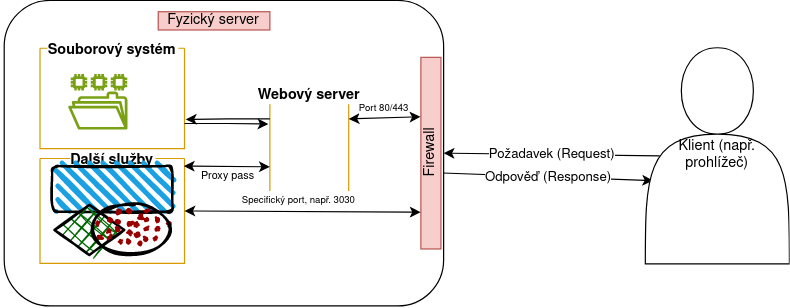
\includegraphics[width=16cm, height=6cm]{files/img/server-client.png}
                \caption{Schéma komunikace client-server}
                \label{fig:client-server}
            \end{figure}

            \textbf{Hosting} je~služba, kterou poskytují \emph{hostingové společnosti}, které mají~\emph{webové servery} a~poskytují na~nich prostor pro~webové stránky (\textbf{Webhosting}) resp.~pro~další služby typu databáze, cloudové úložiště, vlastní aplikace nebo i~vlastní fyzický server (\textbf{Serverhosting})~\cite{dockernginxperformance}.

        \section{Domain Name Server}
            \acrdefprint{DNS}{Domain Name Server}, někdy také \emph{Domain Name System}, je~systém, který překládá doménová jména na~IP adresy. To~umožňuje, uživatelům používat lidem čitelná \emph{doménová jména} namísto \emph{IP~adres} cílového serveru, které jsou pro~uživatele těžko zapamatovatelné.
            
            Díky \acrshort{DNS} např.~oblíbený český vyhledávač namísto \emph{IP~adresy} \texttt{77.75.79.222} najdeme na~čitelné adrese \texttt{Seznam.cz}.

            \textbf{Doménové jméno} je~složeno ze~tří částí. První část je~\emph{subdoména}, která je~volitelná. Druhou částí je~\emph{doména} (2.\,řádu), která je~povinná a~třetí část je~\emph{doména nejvyššího řádu} (\acrdefprint{TLD}{Top Level Domain}{TLD}, která je~také povinná a~může jít např.~o~národní koncovky nebo~některou ze~specifických domén (např.~\texttt{.edu, .org}. \acrshort{TLD} mohou být např.~\texttt{.com}, \texttt{.cz}, \texttt{.eu}, \texttt{.org}. Doménové jméno je~v~procesu nazývaném \textbf{DNS resolve} přeloženo zpět na~\emph{IP adresu}~\cite{tld:mdn}.
        
            \begin{figure}
                \centering
                \begin{tabular}{l l l l l}
                    \textcolor{red}{\texttt{protokol}} &
                    \textcolor{blue}{\texttt{subdoména}} &
                    \textcolor{green}{\texttt{doména}} &
                    \textcolor{orange}{\texttt{TLD}} &
                    \textcolor{purple}{\texttt{?query}}\\

                    \textcolor{red}{\texttt{https}}:// &
                    \textcolor{blue}{\texttt{robot}} &
                    . \textcolor{green}{\texttt{killermachine}} &
                    . \textcolor{orange}{\texttt{com}} &
                    / \textcolor{purple}{\texttt{?znicitlidstvo=false\&parametr=42}}
                    
                \end{tabular}
                \caption{Složky URI}
                \label{slozeni-uri}
            \end{figure}

            \textbf{DNS Resolve} je~proces překladu doménového jména na~IP adresu. Když si~uživatel vyžádá nějaké doménové jméno, prohlížeč se~připojí k~\emph{DNS} a~požádá jej o~překlad doménového jména na~IP adresu. \emph{DNS} odpoví \emph{IP~adresou}, kterou prohlížeč použije pro~navázání spojení se~serverem.

            Když~je do~prohlížeče zadáno doménové jméno, prohlížeč se~pokusí najít \emph{IP~adresu} ve~vlastní \emph{DNS cache}, kam si~ukládá již navštívené weby. Pokud adresu nenajde, připojí~se k~nejbližšímu DNS serveru a~požádá o~poskytnutí překladu jej a~uloží si~\emph{IP adresu} do~\emph{cache}. Pokud \emph{DNS server} adresu nemá, zeptá se~nadřazeného \emph{DNS serveru}~atd.
            
            Nejbližší \acrshort{DNS} bývá poskytovatel připojení k~internetu (\acrdefprint{ISP}{Internet Service Provider}), který má~uloženy \emph{IP} adresy serverů, na~které v~minulosti zákazníci přistupovali. Pokud~záznamy ještě nemá, zeptá se~prohlížeč nadřazeného \emph{DNS serveru}, resp.~zašle požadavek na~adresu nastaveného \acrshort{DNS}. Postupně~se tedy zeptá \acrshort{ISP}, správce národní domény (\emph{CZ.NIC}) a~\emph{kořenového DNS serveru} (\emph{Root DNS server}), který má~uloženy všechny \emph{IP adresy} serverů, které jsou~na~internetu.

            \textbf{DNS Záznamy} (\textbf{DNS Entries}) může~upravovat vlastník domény prostřednictvím \textbf{doménového registrátora}. To~umožňuje přesměrovat doménu na~jiný server, nebo~přidat další záznamy, jako např.~\emph{MX} záznamy, které používá e-mailová služba pro doručování e-mailů~\cite{dns:mdn}.
        
        \section{Model View Controller}
        \label{MVC}
            Významným bodem vývoje aplikací je~rozšíření používání architektury \acrdefprint{MVC}{Model View Controller}. Tato architektura odděluje \textbf{logiku aplikace} od~jejího \textbf{zobrazení}. To~umožňuje vývoj funkční části aplikace nezávisle na~jejím \emph{zobrazení}.

            Podle modelu \acrshort{MVC} má~aplikace 3~složky. \textbf{Model}, který se~stará o~úschovu a~manipulaci s~daty, \textbf{controller}, který zprostředkuje komunikaci mezi \emph{modelem} a~\emph{zobrazením}, a~\textbf{view}, který se~stará o~výsledné zobrazení dat.
            
            Díky tomu je~možné mít~jednu aplikaci, která bude mít~různá \emph{zobrazení} (\emph{view}), zatímco data čerpá pouze z~jednoho zdroje. Např.~webová stránka, mobilní i~desktopová aplikace (\emph{zobrazení}) mohou využívat týž~\acrshort{BE} (\emph{model}).
            
            Moderní aplikace díky tomu mohou snížit zátěž na~server, jelikož část aplikace, která se~stará o~zobrazení, běží na~straně klienta a~mezi nimi probíhá pouze výměna dat~\cite{MVC}.

        \section{Frontend, Backend}
            Dnešní aplikace je~možné díky architektuře \emph{MVC} rozdělit na~\textbf{frontend} a~\textbf{backend}, které spolu komunikují a~plní funkce aplikace ale jinak zůstávají oddělené.

            Díky \acrshort{MVC} je~takto možné vývoj aplikace rozdělit mezi tým~vývojářů, kde každý může pracovat na~jiné části aplikace a~každá část aplikace má~své rozhraní, takže mohou pracovat téměř nezávisle na~sobě.

            \acrdefprint{BE}{Backend} je~část aplikace, která běží na~serveru a~zpracovává nebo~poskytuje data \acrshort{FE}. Spolupracuje s~databází (\emph{Modelem}), souborovým systémem a~dalšími službami, které jsou potřeba pro~fungování aplikace. \acrshort{BE} může být~napsán v~různých jazycích~\cite{Dorman:webmappingajax, Zimmerman2023:howtowritebetter}, např.~PHP, Java, C\#, Go, Javascript, C++\dots

            \acrdefprint{FE}{Frontend} je~část aplikace, kterou vidí uživatel, např.~prostřednictvím prohlížeče. Stará se~o zobrazení (\emph{view}) a~interakci s~uživatelem (\emph{controller}) a~komunikuje s~\acrshort{BE}, zejména pomocí asynchronních požadavků na~server. Je~napsán většinou v~\acrshort{HTML}, \acrshort{CSS} a~\acrshort{JS}.

        \section{Javascript Object Notation}
            \acrdefprint{JSON}{Javascript Object Notation}~je~formát pro~uložení strukturovaných dat. Je~to~textový formát čitelný pro~člověka i~pro~stroj. Používá se~ke~strukturovanému ukládání a~přenosu dat. Dříve byl~hojně využíván formát \acrdefprint{XML}{Extended Markup Language}, který vznikl v~r.~1998 jako formát pro jednoduchou výměnu dat a~který je~podobný struktuře \acrshort{HTML}. Ostatně \acrshort{XML} stále používá spousta aplikací, zejména aplikace státní správy.

            Formát \emph{JSON} je~podobný zápisu objektů v~\emph{Javascriptu}. Obsahuje dvojice \emph{klíč-hodnota}, které jsou odděleny dvojtečkou. Klíčem je~řetězec, který obvykle popisuje, jaká data jsou v~něm uložena, a~hodnota může být číselná, textová, logická hodnota, pole nebo další vnořená struktura dat.
            
            Práce s~formátem \emph{JSON} je~pohodlnější než s~formátem \acrshort{XML}, jelikož je~jednodušší a~čitelnější a~vyžaduje méně kódu, jak na~straně \emph{serveru}, tak na~straně klienta. Jde~tedy~celkově i~o~úspornější formát pro~zápis strukturovaných dat a~jejich~přenos~\cite{Dorman:webmappingajax}.

        \section{Asynchronous Javascript Request}
            \acrfull{AJAX} je~technologie, která umožňuje \emph{asynchronní} komunikaci, např.~mezi \acrshort{FE} a~\acrshort{BE}. To~znamená, že~při~každém požadavku na~\emph{server} se~stránka nemusí znovu načítat, ale použije se~\acrshort{AJAX}, jsou~načtena požadovaná data ze~serveru a~změní se~ve~stránce.

            Metody \emph{Javascriptu} (resp.~\emph{WEB APIs}), umožňující \emph{asynchronní} požadavky na~server, jsou \textbf{Fetch} a~\acrdefprint{XHR}{XMLHttpRequest}. \acrshort{AJAX} využívá různé \acrshort{HTTP} metody, jako GET, POST, PUT, DELETE, PATCH. Tyto metody se~používají pro~odlišení typu požadavku.~\cite{ajax:mdn, Dorman:webmappingajax}.
            
            Je~také možné využít komunikaci přes~\acrshort{WS} nebo~nedávno~přidané~\acrshort{SSE}~\cite{whatwg_sse, sse:mdn}

        \section{Application Interface}
            \acrdefprint{API}{Application Programming Interface} je~rozhraní, které umožňuje komunikaci mezi~aplikacemi. V~případě webových aplikací se~jedná o~rozhraní mezi \acrshort{FE} a~\acrshort{BE}. Některá \emph{rozhrání} jsou určena ke~komunikaci mezi aplikacemi nebo~dokonce s~\emph{hardwarem}.
            
            Někerá \acrshort{API} jsou veřejná a~umožňují komunikaci s~aplikacemi třetích stran. Např.~\acrshort{API} Google Firebase, Microsoft Azure nebo Amazon Web Services umožňují tvorbu tzv.~Serverless aplikací, kde~vývojář tvoří pouze \acrshort{FE} a~o~zbytek se~stará externí služba. To~umožňuje vývojářům se~soustředit na~vývoj aplikace a~nemusí se~starat o~infrastrukturu, která je~potřeba pro~běh aplikace.

            V~dnešní době jsou nejrozšířenější formou tzv.~\acrshort{REST}~\acrshort{API} a~\emph{GraphQL}. Pro komunikaci mezi interními aplikacemi se~často používá protokol \emph{SOAP}. Různý hardware používá k~ovládání také~\emph{UART} nebo~\emph{SPI}.

            Velice oblíbená je~metoda také~\emph{gRPC} (\emph{Google Remote Procedure Call}), která je~založena na~protokolu HTTP/2 a~používá binární formát \emph{Protocol Buffers}. \emph{RPC} je~zkratka pro~\emph{Remote Procedure Call} a~funguje tak, že spouští vzdálené funkce, které jsou na~serveru.
            
            Výhodou \emph{gRPC} je, že autor aplikace pouze definuje služby a~jejich rozhraní a~\emph{gRPC} vygeneruje veškerý potřebný kód pro~jazyk, který používáme. Také je~díky efektivnější komunikaci rychlejší než~jiné~přístupy. Bohužel je~k~jeho použití nutné se~naučit novému přístupu k~přenosu~dat a~jazyku definice služeb \emph{protobuf}~\cite{thenewstackBuildRealWorld}.

        \section{Representational state transfer}
            \acrdefprint{REST}{Representational State Transfer} je~standard, který definuje způsob komunikace mezi klientem a~serverem. V~dnešní době je~díky své~jednoduchosti a~rozšířenosti nejčastěji používanou architekturou pro~tvorbu webových rozhrání. Každý zdroj, se~kterým pracujeme má~vlastní \emph{Endpoint} (vlastní adresu) a~akce, kterou je~potřeba provést, je~určena \emph{HTTP metodou}.
            
            \acrshort{REST} je~bezstavový, což~znamená, že~každý požadavek je~nezávislý na~předchozím, server si~neukládá data v~závislosti na~připojeném klientovi. To~umožňuje jednodušší testování a~ladění aplikace a~trochu snižuje zátěž serveru. Také to~ale~přináší některé výzvy a~omezení, které je~potřeba řešit. Proto je~sice při~tvorbě \acrshort{REST}~\acrshort{API} doporučeno omezit využití ukládání dat vázaných na~konkrétní relaci, nicméně nástroje typu \textbf{Cookies} nebo \textbf{Session} je~v~případě potřeby možné využívat.
            
            \acrshort{REST} definuje, jaké \emph{HTTP metody} se~používají pro~komunikaci, a~každé přiděluje určitý význam. Mezi nejčastěji používané metody patří \emph{GET}, \emph{POST}, \emph{PUT}, \emph{DELETE} a \emph{PATCH}. Metoda je~uložena v~hlavičce \acrshort{HTTP} požadavku. Význam jednotlivých \emph{HTTP metod} je~následující:
            
            \begin{description}
                \item[GET] slouží pro~získání dat ze~serveru,
                \item[POST] pro~odeslání dat na~server,
                \item[PUT] pro~úpravu dat na~serveru,
                \item[DELETE] slouží pro~smazání dat ze~serveru,
                \item[PATCH] potom pro~úpravu části dat na~serveru.
            \end{description}

            Souhrnně se~těmto operacím říká \emph{CRUD operace}. \textbf{CRUD} je~zkratka pro~\textbf{Create}, \textbf{Read}, \textbf{Update} a~\textbf{Delete}.

            Kromě metod \emph{GET} a~\emph{DELETE} se~v~těle \emph{HTTP požadavku} mohou zasílat také data v~textové formě, např.~formátu~JSON. Během přenosu je~tělo požadavku zašifrováno. V~případě požadavku \emph{GET} se~data vkládají do URL adresy, nejsou šifrována a~mají velikost limitovanou maximální délkou \emph{URL adresy}, který je~server schopen zpracovat. Specifikace \acrshort{HTTP} neuvádí žádnou maximální délku, ale v~praxi je~limitována prohlížeči a~serverem. \cite[3.2.1]{ietf-httpbis-messaging-03}

        \section{GraphQL}
            Naproti \acrshort{REST}u má \textbf{GraphQL} pouze jeden \emph{endpoint}. \emph{GraphQL} je~jazyk, který umožňuje klientovi specifikovat, jaká data chce klient získat. To~umožňuje získat všechna potřebná data v~jednom požadavku, což~může být~výhodné, pokud na~zařízení je~pomalé připojení nebo~používá~mobilní data, kdy~je~potřeba stahovat co~nejméně dat a~snížit počet požadavků na~server.

            Na~druhou stranu je~implementace \emph{GraphQL} složitější než~implementace \acrshort{REST}, protože je~potřeba implementovat \emph{GraphQL} server, umí zpracovat požadavky od~klienta. Každá položka, kterou je~potřeba zpřístupnit, navíc musí mít vlastní~\emph{resolver} v~\emph{GraphQL} schématu, který zpracuje požadavek a~vrátí data. To~zároveň vytváří větší zátěž na~serveru, protože je~potřeba pro~každou položku spustit vlastní funkci a~to~je v~případě větších datových objektů a~přístupu do~databáze neefektivní~\cite{Herrera:restgraphql, Dorman:webmappingajax}.

        \section{Zabezpečení}
            Vystavením aplikace na~internetu se~\acrshort{API} vystavuje~nebezpečí útoku a~prolomení zabezpečení. Proto je~potřeba v~aplikaci na~zabezpečení myslet a~v~žádném případě nespoléhat pouze na~sílu zabezpečení knihoven 3.\,stran, které používáme.
            
            To~znamená, že~je~potřeba zabezpečit \acrshort{API}, databázi a~další služby, které aplikace využívá. Je~nutné zvážit např.~jaké služby je potřeba mít veřejně dostupné a~ke~zbytku služeb zamezit přístup z~internetu pomocí \textbf{firewallu}. K~ostatním službám, ke~kterým je~potřeba mít soukromý přístup potom přistupovat pomocí tzv.~\textbf{SSH tunelu}, ideálně za~použití \textbf{SSH klíče}. Navíc je~nutné udržovat systémy aktuální s~nejnovějšími bezpečnostními aktualizacemi~\cite{graham2021ethical, Dorman:webmappingajax}.
            
            \subsection{Hashování}
                \textbf{Hashování} je~proces, při~kterém ze~zadaných dat použitím určitého algoritmu vytvoří řetězec jiný, tak, že~z~něj nelze získat původní data. To~se~používá např.~při~ukládání hesel, kdy heslo uživatele není uloženo v~původní čitelné podobě, ale jako \textbf{hash}. Při~přihlášení pak~stejnou \emph{hashovací} funkcí~zadané heslo ověří s~uloženým \emph{hashem}, jelikož \emph{hashovací funkce} pro~dva~stejné vstupy vrací totožné výsledné \emph{hashe}. Pokud se~shodují, uživatel byl~úspěšně ověřen a~tedy přihlášen.
                
                Pokud se~někomu podaří z~\emph{hashe} získat původní data (heslo), nebo dokáže najít způsob, jak z~různých dat vygenerovat stejný \emph{hash}, považuje~se algoritmus za~prolomený a~měl~by se~přestat používat.
                
                K~\emph{hashování} hesel se~navíc používá tzv.~\textbf{salt (sůl)}, což~je~náhodně vygenerovaný řetězec uložený s~heslem (ve~formě \emph{hashe}) v~databázi, který se~přidává k~heslu před \emph{hashováním}. Protože pro~každou kombinaci by~měl algoritmus generovat jiný \emph{hash}, je takto ztíženo zjištění původního hesla i~v~případě úniku \emph{hashe} na~veřejnost~\cite{graham2021ethical}.
        
            \subsection{Šifrování}
                Při~\textbf{šifrování} je~naopak potřeba získat původní data z~\textbf{šifrovaného textu} (\textbf{ciphertext}). K~šifrovacímu algoritmu je~potřeba vygenerovat klíč, kterým se~šifrují i~dešifrují data. Algoritmus za~pomocí klíče data zašifruje. Při~dešifrování týž algoritmus pomocí klíče \emph{šifrovaný text} dešifruje do~původní podoby.

                Z~hlediska zabezpečení webové aplikace pak~existují dva základní procesy. \emph{Autentizace} a~\emph{autorizace}~\cite{graham2021ethical}.

            \subsection{Autentizace}
                \emph{Autentizace} je~proces ověření identity uživatele. To~znamená, že~uživatel musí dokázat, že~je~tím, za~koho se~vydává. To~je~možné udělat pomocí hesla, certifikátu, který uživatel má, nebo pomocí externí služby, která identitu ověří a~potvrdí ji.
                
                V~případě \acrshort{API} se~jedná o~ověření, že~požadavek přišel z~naší aplikace a~ne z~jiného zdroje, např.~od~útočníka. Do~aplikace se~přidává tajný klíč, který slouží k~identifikaci aplikace a~při každém požadavku na~\acrshort{BE} si~ověřuje \emph{autenticitu} požadavku. Na~to~existují různé metody, např.~využití \acrshort{JWT}.
                
                Do~\acrshort{FE} aplikace je~obvykle vložena dvojici tajných klíčů, které backendu řeknou, že~jde skutečně o~autorizovanou aplikaci, která má~k~backendu povolený přístup. Také je~možné pro~větší bezpečnost přístup omezit pouze na~konkrétní IP~adresy, ze~kterých je~možné se~připojit a~\acrshort{URI}, ze~které lze požadavek odeslat.

                Při~\emph{autentizaci} aplikace je~důležité kontrolovat také jestli byl~požadavek vytvořen naší aplikací na~našem webu a~další informace, které by~mohly odhalit nepovolený přístup. Při~každém požadavku je~pak potřeba ověřit, že~\emph{token} nebyl změněn a~přichází stále ze~stejné aplikace a~stejné \emph{IP adresy}, jako při~první \emph{autentizaci}~\cite{graham2021ethical}.
            
            \subsection{Autorizace}
                Autorizace je~proces ověření oprávnění uživatele k~manipulaci s~konkrétním zdrojem. Ověřujeme, zda~má~uživatel oprávnění k~provedení určité akce, např.~úprava, resp.~smazání příkladu. Je~nutné vzít v~potaz \emph{uživatelskou roli} (tj.~administrátor, uživatel, návštěvník\dots), kterou uživatel má~ve~vztahu k~aplikaci a~k~danému zdroji.
                
                Je~potřeba zkontrolovat vlastnictví nebo~přidělená oprávnění (\uv{může uživatel článek jen zobrazit nebo i~upravovat?}). Např.~pokud je~uživatel autorem příladu, může s~ním libovolně manipulovat. Pokud příklad vytvořil někdo jiný, musí k~úpravě dostat oprávnění~\cite{graham2021ethical}.

            \subsection{JSON Web Token}
                Hojně používaná metoda zabezpečení je~\acrdefprint{JWT}{JSON Web Token}. Jedná se~o~formát \textbf{textového řetězce} (tzv.~\textbf{tokenu}), který obsahuje informace o~uživateli a~aktivním stavu aplikace ve~vztahu k~němu. \emph{Token}~se~při~každém požadavku posílá v~hlavičce požadavku a~umožňuje tak ověřit, že~požadavek přichází z~naší aplikace a~nejde o~nepovolený přístup.
                
                Při~\emph{autentizaci} se~vygeneruje \emph{token} (řetězec znaků), který se~při~každém požadavku na~server posílá v~hlavičce požadavku. Data v~tokenu jsou kódována ve~formátu \textbf{base64} a~podepsána šifrovacím klíčem, takže je~nelze, bez~znalosti klíče, změnit, protože jakákoliv změna v~datech znamená změnu \emph{podpisu}. Do~tokenu se~přidávají data, která je~potřeba uchovat nebo jsou~využita k~dodatečné kontrole. Je~důležité do \emph{tokenu} neukládat žádná citlivá data, jelikož formát \emph{base64} není šifrovaný. 
                
                V~případě změny nebo~nepřesnosti v~datech \emph{tokenu} se~díky podpisu \emph{token} stává neplatným, což~umožňuje ověřit, že~token byl vytvořen serverem a~ne někým jiným. Zároveň v~datech \emph{tokenu} je~možné mít informace o~aktuálně přihlášeném uživateli, a~další kontrolní informace, jako~délka platnosti \emph{tokenu}, \emph{IP~adresa požadavku}, \emph{typ zařízení} a~\emph{doména}, ze~které byl požadavek na~jeho~vytvoření prvně odeslán.\\

                \acrshort{JWT} sestává ze~tří částí, které jsou odděleny tečkou.
                
                \begin{description}
                    \item[Hlavička (header)] obsahuje informace o~typu tokenu a~typu šifrování podpisu.
                    \item[Tělo tokenu (body)] obsahuje data, která je~potřeba uchovat (\emph{payload}).
                    \item[Podpis (signature)] zajišťuje kontrolu, že~token nebyl během cesty na~server změněn.
                \end{description}

                Všechny tři~části jsou zakódovány pomocí metody \emph{Base64} a~odděleny tečkou. Výsledný token je~také textový řetězec, který je~možné přenášet v~hlavičce \emph{HTTP~požadavku}.

                Funkci \acrshort{JWT} v~praxi lze~vidět na~schématu \ref{model-jwt}.

                \begin{figure}
                    \centering
                    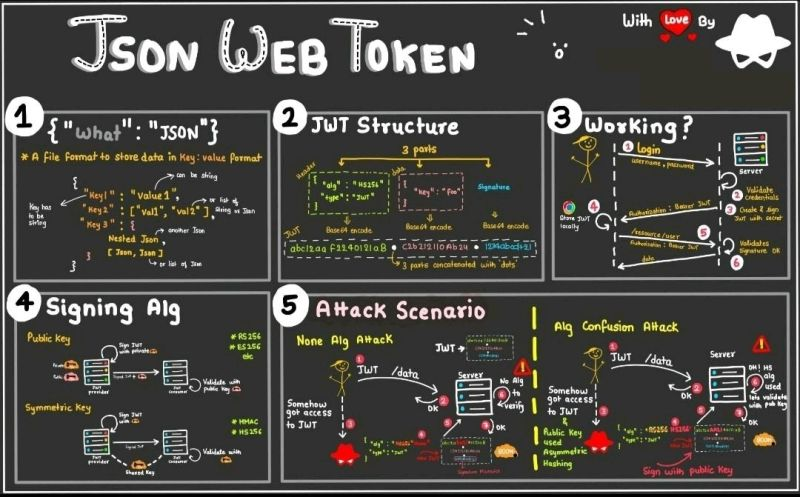
\includegraphics[width=.9\linewidth]{./files/img/jwt.jpg}
                    \caption{Použití JWT v~praxi}
                    \label{model-jwt}
                \end{figure}

                Jednou z~výhod \acrshort{JWT} je~možnost přenositelnosti. Token může být~vytvořen na~jednom serveru a~ověřen na~jiném, který má k~dispozici daný klíč (\cite{ieee:jwt}). Je~možné tak např.~umožnit jednotné přihlášení v~rámci několika služeb. \acrshort{JWT}~není vázán na~symetrické šifrování a~kvůli přenositelnosti se~často využívá \emph{asymetrické šifrování}, kde hlavní server má~tzv.~\textbf{privátní klíč} (\textbf{private key}) a~další účastnící mají svůj~vlastní \textbf{veřejný klíč} (\textbf{public key}), odvozený od~privátního, kterým ověřují, že~byl~token vytvořen na~správném serveru~\cite{miguelgrinbergJSONTokens}.
                
                Díky \emph{asymetrickému šifrování} je~možné vytvořit více \emph{veřejných klíčů} a~přidělit je~různým službám, které je~pak mohou používat pro~ověření \emph{tokenu} z~původního \emph{serveru}.

                Formát \emph{Base64} je~kódování, které se~používá pro~přenos dat, nikoliv pro~zabezpečení. Bezpečnost \acrshort{JWT} je~zajištěna pouze podpisem, který zaručuje integritu dat. Data ale~může přečíst kdokoliv, kdo získá~přístup k~tokenu. Proto je~důležité do~tokenu ukládat pouze data, která jsou nezbytně nutná a~neobsahují citlivé informace. K~šifrování dat a~ostatních částí \acrshort{JWT} vznikly navazující standardy\,--\,\textbf{JWE}, \textbf{JWS}, \textbf{JWA} nebo~\textbf{JWK}.~\cite{jwtesak, graham2021ethical}

            \subsection{Structured Query Language}
            \acrdefprint{SQL}{Structured Query Language} je~jazyk, používány pro~manipulaci s~daty uloženými v~rámci relačních databází. \acrshort{SQL} je~deklarativní jazyk, což~znamená, že~při~vytvoření dotazu popíšeme, jaká data je~potřeba získat, a~ne jakým způsobem. \acrshort{SQL} je~standardizovaný jazyk, který je~podporován většinou relačních databází. Pomocí \acrshort{SQL} se~zapisují tzv.~\textbf{SQL dotazy} (\textbf{SQL Query}), které mohou ukládat, načítat, upravovat nebo~mazat data v~databázi~\cite{laurencik2018sql}.

            \subsection{SQL Injection}
                \emph{SQL Injection} je~zřejmě nejčastější typ útoku, při~kterém útočník vloží kus~\emph{SQL dotazu} do~neošetřeného uživatelského vstupu (např.\,vstupní pole pro~email) a~pokud jej~autor aplikace neošetří, je~místo zpracování vykonán společně se~zbytkem dotazu. To~může vést k~získání citlivých dat, jejich změně nebo~smazání. Může např.~dojít ke~změně hesla administrátorského účtu a~tím získání přístupu ke~chráněným datům.

                Proto je~nutné data od~uživatele vždy ošetřit a~v~ideálním případě použít navíc tzv.~\emph{Parametrizované dotazy} (\emph{Prepared statements}). Při~použití \emph{parametrizovaných dotazů} se~do~dotazu nevkládají přímo data, ale na~místo, kam~patří data je~vložený tzv.~\emph{Zástupný symbol} (\emph{placeholder}), který je~poté nahrazen ošetřenými (\emph{escapovanými}) daty tak, aby~nebylo možné případný vložený příkaz provést. Zástupný symbol v~SQL představuje otazník \uv{\texttt{?}} nebo v~případě pojmenovaných hodnot název proměnné za~dvojtečkou \uv{\texttt{:nazev}}~\cite{graham2021ethical}.
                
                Např.~dotaz na~změnu emailové adresy, který by~v~případě neošetření umožnil útočníkovi získat administrátorský přístup do~aplikace, by~mohl vypadat, jako v~ukázce \ref{model-sql-injection}.:
                \begin{code}
                    \centering
                    \begin{minipage}{0.48\textwidth}
                        \begin{minted}{go}
id := 42
// nebezpečný vstup od uživatele
email := "mujmejl@seznam.cz', role='admin"
// přímé spuštění dotazu
DB.Exec("UPDATE users SET email = '" + email + "' WHERE id = " + id)
                        \end{minted}
                        \begin{minted}{sql}
-- výsledný spuštěný dotaz, který by umožnil útočníkovi získat administrátorský přístup
UPDATE users SET email = 'mujmejl@seznam.cz', role='admin' WHERE id = 42
                        \end{minted}
                        \subcaption{Neošetřený řetězec vložený do \acrshort{SQL}}
                    \end{minipage}
                    \begin{minipage}{0.48\textwidth}
                        \begin{minted}{go}
id := 42
// nebezpečný vstup od uživatele
email := "mujmejl@seznam.cz', role='admin"
// příprava dotazu pomocí "prepared statements"
DB.Exec("UPDATE users SET email = ? WHERE id = ?", email, id)
                        \end{minted}
                        \begin{minted}{sql}
-- ošetřený (escapovaný) dotaz, který by pouze vložil do databáze nevalidní emailovou adresu
UPDATE users SET email = 'mujmejl@seznam.cz\', role=\'admin', WHERE id = 42'
                        \end{minted}
                        \subcaption{Ošetření SQL injection pomocí prepared statement}
                    \end{minipage}
                    \caption{SQL injection a jeho ošetření}
                    \label{model-sql-injection}
                \end{code}

                Samozřejmě v~příkladu není vstup nijak ošetřen a~k~přijetí takové hodnoty do~pole \texttt{email} by~nemělo vůbec dojít, jelikož nejde o~validní emailovou adresu. Proto je~potřeba vstupní data v~aplikaci ošetřovat nejméně na~2~místech. Všechna vstupní data a~parametrizované dotazy. Také je~dobré zavést kontrolu~před odesláním na~straně uživatele, nicméně na~to~nelze spoléhat, jelikož lze~jednoduše obcházet odeslání dat, tj.~kontrola na~straně uživatele je~především vizuální feedback a~pokyn pro~zadání správné formy dat uživatelem.
                
                Další kontroly vstupních dat mohou probíhat i~na~úrovni databáze. To~už ale~je na~uvážení autora konkrétní aplikace. \cite{w3s:SQLInjection, itnetwork:SQLInjection}

            \subsection{Cross Site Scripting}
                \acrdefprint{XSS}{Cross Site Scripting} je~typ útoku, při~kterém útočník vloží do~uživatelského vstupu kód, který se~při~načtení stránky spustí. To~může vést k~získání citlivých dat, přesměrování na~jinou stránku nebo~k~jiným nežádoucím akcím.

                Možnou ochranou před tímto typem útoku je~nahrazení znaků, které~mohou způsobit problémy, za~jejich \emph{HTML entity}, kde~je~potřeba např.~znaky jako~\texttt{<} nahradit za~\texttt{\&lt;}, \texttt{>} za~\texttt{\&gt;}, \texttt{\&} za~\texttt{\&amp;}~apod. Takové \emph{HTML entity} prohlížeč vykreslí uživateli a~nezpracovává je~jako~funkční kód.
                
                Možností je~také využít specializované knihovny, které toto ošetření provedou samy, a~není nutné řešit otázky, které znaky je~nebo~není potřeba ošetřovat, např.~\emph{DOMPurify} nebo~\emph{sanitize-html}~\cite{medium:XSS}.

                Jelikož v~projektu používám \emph{React}, který využívá \emph{JSX}, je~tento typ útoku téměř vyloučen. \emph{JSX} totiž neumožňuje vkládat přímo \acrshort{HTML} kód, ale~pouze textové řetězce, které se~při~načtení stránky zobrazí.

                Existují ale výjimky a~to~použití funkce \texttt{eval}, která umožňuje spustit \acrshort{JS} kód z~řetězce (textové proměnné), a~přímé vkládání neošetřeného vstupu pomocí vlastnosti \texttt{dangerouslySetInnerHTML} nebo~jí podobných, které se~přímo přepíšou do~kódu, např.~\texttt{href}, \texttt{OnClick}~apod. Tyto vlastnosti ale~vývojáři používají s~vědomím rizika~\cite{reactJSX}.

        \section{Testování}
            Testování je~důležitou součástí vývoje aplikace a~černé svědomí velké části vývojářů. Testování je~časově náročné a~vývojáři se~mu~často vyhýbají, protože je~potřeba vytvořit sadu testů, které pokryjí co~nejvíce možných scénářů, které mohou nastat.
            
            Zejména automatickým testováním je~možné ušetřit spoustu času, který bychom jinak strávili ručním testováním aplikace nebo při hledání chyb, které se~objevily po~změnách v~kódu aplikace. Automatické testování umožňuje vytvořit sadu testů, které je~možné spustit při~každé změně aplikace a~ověřit si~tak, že~aplikace stále funguje správně. Pokud je~daný jazyk navíc \emph{dynamicky typovaný}, je dobré mít~nástroj na~kontrolu správnosti použití funkcí~\cite{compilers, itnetworkBestPractices}.
            
            Např.~při~změnách základní funkcionality je~dobré otestovat, že~i~po~změnách fungují stále stejně. Zejména se~testují tzv.~\emph{čisté funkce} (\textbf{pure function}), což~jsou funkce, které nemají žádné \textbf{vedlejší efekty} (přímo neovlivňují výstupní data a~stav programu) a~pro~stejný vstup vždy poskytnou (vrací) stejný výsledek. Takové testování se~nazývá \emph{unit testing}.
            
            V~každém programovacím jazyce jsou potřeba nástroje pro~automatické testování. Např.~v~případě \emph{Javascriptu} to~jsou~např.~\textbf{Jest} nebo~\textbf{Mocha}. Jazyk \emph{Go}~má~vestavěný nástroj pro~automatické~testování, který se~nazývá \textbf{go~test}.
            
            Pro~testování React aplikace budu~používat \emph{Jest}. Pro~testování backendu potom zmíněný \emph{Go~test}~\cite{jestjsTestingReact}.
            
            \subsection{Testování API}
                Pro~testování \acrshort{API} existují nástroje, které umožní vytvářet požadavky bez~nutnosti mít~dokončenu \acrshort{FE} část. Mezi nejznámější patří \textbf{Postman} nebo~\textbf{Insomnia} atd.
                
                Tyto~nástroje navíc většinou nabízejí možnost vytvořit si~sadu automatických testů, které je~možné spouštět při~sestavování aplikace v~\emph{Dockeru} a~automaticky si~tak~před~kompilací celého programu ověřit, že~jednotlivé součásti \acrshort{API} stále funguje správně, např.~jsou dostupné všechny \emph{endpointy}.

                K~tomuto účelu použiji nástroj \emph{Postman}, jelikož v~době psaní této práce nástroj \emph{Insomnia} neumožňuje přímé psaní testovacích skriptů. 
                
                S~nastaveným testovacím skriptem si~ukládám nový \emph{token} a~při~následujícím požadavku jej~posílám v~hlavičce požadavku. Tímto způsobem mohu~testovat \acrshort{BE}, bez~omezení bezpečnostních opatření.

            \subsection{Testování frontendu}
                Pro~testování \acrshort{FE} budu používat knihovnu \emph{Jest}, kterou na~testování používá např.~\emph{Facebook}. Testovat~bude potřeba \emph{čisté funkce}, ale také \emph{komponenty}. \emph{Komponenty} se~testují pomocí tzv.~\textbf{snapshotů}, které umí~porovnat vykreslenou komponentu s~předchozí zapamatovanou verzí. Pokud se~liší, test selže a~je~potřeba zkontrolovat, zda~je~změna v~pořádku nebo~\emph{snapshot} obnovit v~nové podobě \emph{komponenty}~\cite{jestjsTestingReact}.

        \section{Continous Integration a Continuous Delivery}
            \textbf{CI/CD} je souhrnný pojem, který označuje průběžnou integraci \acrdefprint{CI}{Continuous Integration} a~průběžné doručení nebo nasazování \acrdefprint{CD}{Continuous Deployment/Delivery}, dvě klíčové praktiky v automatizaci procesů vývoje softwaru.

            \textbf{CI} zahrnuje automatické spouštění sady testů po každé změně kódu v repozitáři, aby se ověřila jeho funkčnost a kompatibilita. Cílem je rychle identifikovat a opravit chyby, což vede k udržení vysoké kvality softwaru. Po úspěšném provedení testů dochází k automatickému sestavení aplikace. Pokud testy selžou, proces CI informuje vývojáře o potřebě oprav a zastaví další postup.

            \textbf{CD} rozšiřuje \emph{CI} tím, že po~úspěšném sestavení aplikace automaticky provede její nasazení na~server. To~umožňuje rychlou dostupnost aktualizované aplikace uživatelům bez~manuálního zásahu, což~zvyšuje efektivitu vývojového procesu a~umožňuje rychlejší reakci na~požadavky trhu~\cite{graham2021ethical}.
	
        \section{Verzovací systém GIT}
            \emph{GIT} vytvořil autor Linuxu \emph{Linus Torvalds} v~roce 2005. Je~to~\textbf{distribuovaný verzovací systém}, tj.~každý vývojář má~lokální kopii celého projektu, tedy může pracovat i~bez~připojení k~internetu a~následně své~změny nahrát na~server, když se~připojí.
            
            Základní funkcí \emph{GITu} je~ukládání změn. Neukládají se~celé soubory pouze změny, které se~udály. Díky tomu je~možné spravovat i~větší projekty, kde spolupracuje více vývojářů zároveň a~po~dokončení části práce a~její~kontrole ji~připojí ke~zbytku kódu, který je~označen za~finální verzi (tzv.~\textbf{release}) aplikace nebo je~na~něm~možné dále pracovat.
            
            Díky verzování je~také možné se~kdykoliv vrátit k~předchozím verzím projektu a~pokračovat ve~vývoji nebo~pracovat na~několika různých problémech zároveň díky \textbf{větvím}. Práci je~možné v~jakémkoliv bodě označit pomocí tagů a~tím~umožnit používat označené místo ve~vývoji.

            Existují služby, které poskytují prostor pro~ukládání \emph{GIT} projektů online, tak~aby~byly zálohované a~přístupné odkudkoliv, jako např.~\emph{GitHub}, \emph{GitLab} nebo~\emph{Bitbucket}. Mimo zmíněné funkce nabízejí možnost vytvářet \textbf{Issues}, pokud narazí na~chybu nebo~má~nápad na~vylepšení. Tímto způsobem může sdělit svůj nápad nebo~chybu v~aplikaci a~případně se~k~ní vrátit později. \emph{Issues} je~také možné přiřadit konkrétnímu vývojáři, který chybu nebo~nápad dostane na~starost nebo~automaticky vytvořit \emph{větev}, na~které bude práce probíhat. Na konci práce vývojář vytvoří tzv.~\textbf{Merge Request}, kde oznámi, jak problém řešil, a požádá o~sloučení nového kódu do~hlavní \emph{větve} projektu. Je~také možné jednoduše zobrazit rozdíly mezi hlavní \emph{větví} a~tou, na~které vývojář pracuje~\cite{gitscmBook}.
            
            \emph{GIT} je~pro~vývoj dnešních aplikací nepostradatelný nástroj.
            
            \emph{Gitlab} je~open--source nástroj pro~správu a~udržování \emph{GIT repozitářů} na~serveru. Podobně jako \emph{Github} nabízí možnosti, jak~kompletně spravovat projekty. Kromě toho je~často používán k~automatizaci testování a~publikaci aplikace na~produkční server (\emph{CI/CD pipeline}, viz~sekce o~\emph{testování aplikací}). Je~možné jej~nainstalovat na~vlastní server a~mít~tak~plnou kontrolu nad~svými daty, čehož~využívá spousta společností, pokud např.~mají více projektů nebo nechtějí svůj kód~ukládat na~cizích serverech~\cite{gitlab:panek2019optimalizace, gitlab:CICD, gitlab:actions}.

            \subsection{Git hooks}
                \textbf{Git hooks} jsou~skripty, které se~spouští při~určité události v~\emph{Gitu}. Je~možné např.~automaticky spustit testy před~každým nahráním změn v~kódu do~repozitáře~\cite{gitscmBook}.

            \subsection{Gitlab Actions}
                \emph{Gitlab Actions} jsou~součástí \emph{Gitlabu} a~umožňují vytvořit sadu procesů (tzv.~\textbf{workflow}), které se~spustí při~určité události, např.~při~nahrání nového kódu do~repozitáře.
                
                \emph{Workflow} se~spouští ve~virtualizačním prostředí (\emph{kontejneru}), který je~vytvořený na~základě \emph{Dockerfile} a~obsahuje prostředí, potřebné pro~sestavení a~spuštění aplikace a~testů. Celý proces se~automaticky spouští na~\emph{virtuálním serveru}, např.~po~nahrání projektu na~\emph{Gitlab} a~nastavuje se~pomocí konfiguračního souboru \emph{.yml}.

                Během procesu se~spustí \emph{kontejner}, ve~kterém se~aplikace sestaví a~spustí se~přednastavené testy. Pokud vše proběhne v~pořádku, aplikace se~automaticky nasadí na~server. Použitím \emph{CI/CD} procesů se~zjednoduší nasazování aplikace a~zrychlí proces~vývoje~\cite{gitlab:actions}.

        \section{Pravidla přístupnosti webu}
                Webové aplikace je~nutné vytvářet přístupné pro~všechny uživatele. Tato pravidla jsou~definována v~\acrdefprint{WCAG}{Web Content Accessibility Guidelines}, které jsou~vydávány organizací \acrdefprint{W3C}{World Wide Web Consortium}.

                V~ČR je~přístupnost webu upravena zákonem č.~99/2019 Sb., o~přístupnosti internetových stránek a~mobilních aplikací veřejného sektoru a~o~změně zákona č.~365/2000 Sb., o~informačních systémech veřejné správy a~o~změně některých dalších zákonů (zákon o~přístupnosti).

                \textbf{Pravidla přístupnosti} zahrnují optimalizaci (přizpůsobení) aplikace pro~hladké použití aplikace osobami se~zrakovými nebo sluchovými vadami, poruchami pohybu~ap. Mají např.~zjednodušit navigaci ve~stránce pomocí klávesnice, či~s~použitím programů na~čtení displeje, zmiňují kontrast prvků ve~stránce pro~lepší čitelnost a~správné použití \textbf{semantických} (\textbf{významových}) prvků \acrshort{HTML} jako~\texttt{<nav>}, \texttt{<header>}, \texttt{<article>}, správně použité úrovně nadpisů a~další~\cite{w3WCAGOverview}.

        \section{Optimalizace pro vyhledávače}
                Důležitou součástí, která souvisí i~s~přístupností je~\acrdefprint{SEO}{optimalizace webu pro~vyhledávače}. Při~\textbf{indexaci} (načtení strukturovaných dat ze~stránky a~jejich zařazení do~vyhledávání). Vyhledávač musí -- stejně jako např.~software pro~čtení obrazovky -- načítat surová data, která si~ukládá do~své~databáze. V~případě, že~jsou data špatně strukturovaná, nebo~nejsou dostatečně popsaná, může dojít k~jejich špatnému zařazení, nebo~k~jejich nezařazení do~vyhledávání. To~může mít~za~následek, že~stránka nebude v~hledání nalezena, nebo~bude nalezena až~na~pozdějších pozicích~\cite{dover2012seo}.

                Důležitými faktory jsou~také zabezpečení webu (\emph{HTTPS}) a~optimalizace pro~mobilní zařízení, nebo správná struktura webu, např.~oddělení navigace od~obsahu (\texttt{<nav><article>}~ap.). Vyhledávače (i~sociální sítě~ap.), např.~\emph{Google} bodují splnění různých kategorií a~podle vlastního algoritmu potom řadí výsledky ve~vyhledávání. Viz~aktualizace algoritmu~\cite{hladis2016aktualizace}.

        \section{Údržba aplikace}
            Údržba aplikace je~důležitá část vývoje. Je~potřeba aplikaci pravidelně aktualizovat a~opravovat chyby, které se~vyskytnou.
            Tedy jde o nejdelší část životního cyklu aplikace. V~této části je~potřeba aplikaci testovat a~opravovat chyby, které se~vyskytnou.
            
            \subsection{Životní cyklus vývoje software}
                \acrdefprint{SDLC}{Software Development Lifecycle} je~označení pro~životní cyklus  software. Jedná se~o~soubor procesů, které se~používají při~vývoji softwaru. Tyto procesy se~opakují v~kolech, které se~nazývají iterace. V~každé iteraci se~vyvíjí část aplikace, která je~následně testována. Vývojáři se~také mohou v~každé iteraci vrátit k~předchozí části a~upravit ji~podle potřeby, případně do~vývoje zapojit zákazníka.

                Ve~většině případů jde~o~opakující se~proces, který se~opakuje až~do~dokončení aplikace. Různé týmy mohou mít~různé požadavky na~vývoj aplikace a~používat jiné modely (metodiky) vývoje, kterých existuje několik;
                
                Nejčastěji je~používán \textbf{Agilní} (\textbf{Agile}) model, který je~založen na~iteracích a~pravidelné komunikaci se~zákazníkem. V~každé iteraci se~vyvíjí část aplikace, která je~následně testována.
                
                Existují ale i~jiné modely vývoje, jako např.~Vodopádový, W-model a další~\cite{sdlc:kadlec2004agilni}.

            \subsection{Sledování chyb nahlášených uživateli}
                Pokud uživatel narazí na~chyby v~aplikaci, měl~by~je~mít~možnost nahlásit. Vývojář má~potom lepší možnost tyto chyby sledovat a~opravit~je.

                Podobný je~i~případ požadavků na~nové funkce. Uživatel by~měl mít~možnost požádat o~novou funkci nebo zlepšení stávajících,
                aby~vývojář mohl aplikaci dále rozvíjet.

            \subsection{Běhové a kompilační chyby}
                \textbf{Kompilace} (\textbf{sestavení}) je~proces překladu zdrojového kódu do~binárního souboru, který je~přímo spustitelný na~procesoru. Při~kompilaci se~kontroluje správnost kódu, datových typů~ap. Případné chyby překladač oznámí vývojáři. Některé chyby může překladač opravit automaticky a~podle závažnosti chyby a~námi zavedených parametrů překlad proběhne v~pořádku nebo se~překlad zastaví a~je~potřeba chyby předem opravit.

                Chyby se~ale mohou projevit až~při~běhu programu. To~jsou chyby, které např.~závisí na~datech, která se~do~programu načítají nebo je~zadává uživatel. Příkladem takové chyby může být špatná práce s~pamětí, která může vést k~přetečení paměti a~následnému pádu programu.

                Na~běhových chybách se~docela často zakládají útoky na~aplikace, proto je~potřeba je~hlídat. Útočník může záměrně zasílat data, která způsobí chybu v~aplikaci, čímž může získat přístup k~systému nebo získat data, ke~kterým by~jinak přístup neměl.

                Důležité pro~opravní chyb je~uvědomit si~jejich příčinu. To~je~často složité, protože chyba se~může projevit až~po~několika krocích nebo pouze za~specifického stavu aplikace~\cite{graham2021ethical}.

                Proto je~nutné aplikaci testovat, chyby zaznamenávat i~se~vstupními daty a~opravovat~je. To~je~důležitá část vývoje aplikace. Jeden z~nástrojů, které efektivní sledování chyb~umožňují, je~\emph{Sentry}.

            \subsection{Sentry}
                \emph{Sentry} je~nástroj, který umožňuje zachytávat chyby za~běhu aplikace. Pomocí webového rozhrání potom může vývojář (nebo jeho tým) sledovat chyby, které se~vyskytly za~chodu~aplikace. \emph{Sentry} umožňuje sledovat chyby v~různých jazycích, jako v~našem případě \emph{Javascript a Go}. Ale funguje i~v~dalších jazycích. Existuje~také modul pro~integraci s~frameworkem \emph{Gin}, což~umožňuje získat i~informace o~\acrshort{HTTP} požadavku a~stavu serveru, který chybě předcházel.
                
                V~každém z~těchto jazyků umožní \emph{Sentry} sledovat chyby specifické pro~daný jazyk a~tím zjednodušit opravu chyb. Např.~v~případě \emph{Javascriptu} umožní sledovat akce, které uživatel provedl před tím, než došlo k~chybě. Chyby z~\acrshort{BE} i~\acrshort{FE} aplikace se~uloží na~jedno místo a~je~tak pro~celý tým jednodušší s~nimi pracovat.

                Díky tomu má~vývojář k~dispozici spoustu informací, které potřebuje k~nalezení, vyvolání a~opravě chyby. \emph{Sentry} také umožňuje přímo vytvářet \emph{úkoly}, na kterých mohou vývojáři pracovat. To~umožňuje vývojářům efektivněji rozdělovat práci na~opravách chyb, které \emph{Sentry} zachytí.

                Informace navíc zůstanou uloženy v~\emph{Sentry} a vývojáři se~k~nim mohou kdykoliv vrátit. \emph{Sentry} je možno integrovat do~různých komunikačních nástrojů, jako např.~\textbf{Slack}, \textbf{Telegram}, \textbf{Whatsapp} nebo~\textbf{Discord}, které se~běžně používají ke~komunikaci ve~vývojových týmech a~upomínka v~případě chyby se~objeví přímo v~komunikačním kanálu týmu.

        \section{Linux a příkazová řádka, Windows Subsystem for Linux}
            Linux je~operační systém, který vytvořil Linus Torvalds v~roce 1991. Jde~o~nejrozšířenější \emph{open--source} operační systém, používaný zejména na~serverech. Je~možné jej ale jednoduše použít také na~\emph{desktopových zařízeních} v~podobě mnoha distribucí (např. Ubuntu, Linux Mint, \dots)
            
            Je~to~také základ pro~mnoho dalších operačních systémů, jako např.~\emph{Android \emph{open--source} project (\emph{AOSP})} od~společnosti \emph{Google}, který na~\emph{jádro OS Linux} přidává funkce pro~použití na~mobilních zařízeních~\cite{AOSP:linux}.
            
            Velikou výhodou je~otevřenost a~možnost upravovat zdrojový kód. To~umožňuje vývojářům nahlížet a~navrhovat změny ke~zlepšení do~jádra \emph{Linuxu}. Výhodou je~také jeho bezpečnost a~svoboda. V~porovnání s~jinými operačními systémy je~bezpečnější a~méně náchylný ke~škodlivým programům, zejména díky pravidlům pro~přístupy k~souborům. V~Linuxu je~navíc za~soubor považováno všechno (konfigurace, procesy, síť i~periférie atd.), což~zabezpečení zjednodušuje - pokud jsou~správně nastavena přístupová oprávnění a~vlastnictví~\cite{medium:LinuxSecure}.

            Nabízí mnoho grafických prostředí, takže si~uživatel může vybrat, jakým způsobem bude~systém používat a~je~možné téměř všechno nastavit tak, jak v~práci potřebuje. Navíc většina nástrojů pro~vývoj aplikací je~vyvíjena pro~Linux, takže je~možné je~používat bez~problémů a~automaticky vše nastavit jedním skriptem z~příkazové řádky. Není také nutné instalovat a~mít~zároveň spuštěno několik různých nástrojových oken, vše je~na~jednom místě.

            Kvůli zvyšujícímu~se počtu vývojářů pracujících na~Linuxu přidala firma Microsoft do~svého operačního systému Windows možnost spouštět aplikace a~příkazy Linuxu pomocí nástroje~\textbf{WSL2 (Windows Subsystem for Linux)}. Jedná se~o~virtuální stroj, který běží na~pozadí a~umožní uživateli Windows používat výhody, které nabízí Linux, např.~má~vývojové nástroje na~jednom místě, místo několika oken, které musí mít~otevřené při~normálním vývoji na~Windows~\cite{WSL2Winning2023}.

        \section{Integrated Development Environment a nástroje pro psaní kódu}
            \acrdefprint{IDE}{Integrated Development Environment} (\textbf{integrované vývojové prostředí}) jsou programy, které umožňují vývojářům psát spouštět a~ladit (tzv.~\textbf{debugovat}) ji~v~jednom prostředí. To~umožňuje vývojářům pracovat efektivněji a~rychleji. V~jednom editoru mají~všechny nástroje, které potřebují k~vývoji aplikace. V~dnešní době existuje spousta \acrshort{IDE}, které se~liší podporovanými jazyky, funkcemi a~vzhledem. Funkcionalitu lze~většinou doplňovat i~o~nové funkce pomocí pluginů.
            
            Mezi nejznámější \acrshort{IDE} patří \emph{Visual Studio Code}, \emph{IntelliJ IDEA}, \emph{Google Atom}, \emph{Netbeans} nebo~\emph{Sublime Text}. Jako \acrshort{IDE} je~možné při~vhodném nastavení označit také konzolový editor \emph{Vim}~\cite{IDE}.
            
            S~pokrokem \emph{umělé inteligence} (\emph{AI}) se~objevují nástroje, které dokáží automaticky opravovat chyby v~kódu, nebo~dokonce přímo na~základě formálního popisu běžným jazykem psát kód za~vývojáře, viz~\cite{pasek:generovanizdroju}. To~ale zatím není možné v~každém jazyce a~je~nutné kód osobně zkontrolovat, protože generativní nástroje mohou vytvořit kód, který je~sice funkční, ale~neefektivní nebo~nečitelný.

            Příkladem nástroje generování kódu může být~např.~\emph{Github Copilot}, který dokáže na~základě komentářů nebo kontextu v~kódu vygenerovat funkční pokračování kódu. Další nástroje jsou např.~\emph{Tabnine}, \emph{Kite} a~další~\cite{sz:AI}.
            
            V~průzkumu \uv{The State Of AI Tools 2023}~(\cite{zerotomasteryStateOfAI}) většina vývojářů odpověděla, že~se~nebojí toho, že~by~je~\emph{AI} v~blízké budoucnosti plně nahradila. Programování je~komplexní proces, který vyžaduje kreativitu a~schopnost řešit problémy různého typu. Využití kódu od~\emph{AI} je~nutné brát s~rezervou~--~učí se~z~kódu, který~vytvořili lidi, takže může být~ovlivněný jejich nedostatky a~\emph{AI} prozatím není~schopná samostatně přemýšlet nad~řešením problému, ale~pouze generovat data na~základě předchozích řešení, která mohou být~chybná či~neefektivní.
            
            Jazykové modely \emph{AI}, jako~\emph{ChatGPT} či~\emph{Google Bard} potom pomáhají zejména ke~konzultaci problémů a~získání nápadů, jak je~vyřešit. Svým způsobem tím~suplují síť webových fór \emph{Stack Overflow}, kde~si vývojáři navzájem radí s~řešením problémů, zejména z~oboru~\emph{IT}. Tyto \emph{AI} nástroje jsou skvělé na~opakované úkoly, jako přepisování struktur dat nebo hromadných příkazů.

            \emph{AI} nástroje typu \emph{ChatGPT} ale poslední dobou ztrácí na~přesnosti. Je~to~díky tomu, že~k~dalšímu učení využívají data přístupná z~internetu, a~to~často i~data generovaná jinými \emph{AI}. Výsledky je~tedy nutné posuzovat kriticky~\cite{computerworld:AI}.

        \section{Mezinárodní lokalizace}
            \acrdefprint{I18n}{Internationalization} je~proces přizpůsobení aplikace pro~různé jazyky a~kultury. To~zahrnuje mimo překlad např.~formát data, měny nebo~jednotky. Standard \emph{I18n} zahrnuje i~různé formy slov, např.~pro~různá množství~\cite{w3Internationalization}.

            Každý znak je~v~počítači reprezentován číslem. V~minulosti používaly počítače k~ukládání znaků kódování \emph{ASCII}, které (z~historických důvodů) obsahovalo pouze 128~znaků (7 bitů v~rozsahu $0$ až $2^7 - 1$). To~znamená, že~bylo možné zobrazit pouze anglické texty a~některá interpunkční znaménka. 
            
            V~dnešní době se~většinově používá kódování \acrdefprint{UTF}{Unicode}, které k~původním 7~bitům (\emph{ASCII}) přidává další, značící, zda daný znak pokračuje dalším \textbf{bajtem}. To~umožňuje zobrazit mnohem více znaků, vč.~např.~čínských znaků nebo~smajlíků, a~tedy překlad aplikace do~různých jazyků a~znakových sad. Na~druhou stranu každý další byte znamená více použité paměti, kterou text zabírá a~počítač také pracuje déle na~zpracování každého znaku.
            
            Proto je~vhodné všechny~zdrojové kódy a~aplikace psát v~Anglickém jazyce, který využívá základní \emph{ASCII} znaky, a~aplikaci pro~uživatele do~jeho~jazyka překládat (\textbf{lokalizovat}). Anglický jazyk je~navíc považován za~mezinárodní jazyk, který je~známý většině uživatelů a~aplikace je~tak~jednodušeji přístupná širší skupině uživatelů.
            
            Webový prohlížeč si~pamatuje preferenci jazyka uživatele a~při~požadavku na~aplikaci zašle i~informaci o~preferovaném jazyce. Webový server pak~zpřístupní uživateli aplikaci ve~vyžádaném jazyce.

            Pro překlad aplikace se~používají \emph{lokalizační soubory}, které obsahují překlady jednotlivých textů aplikace. Každý jazyk má~svůj soubor, který se~načítá při~spouštění aplikace. Pokud překlad není nalezen, použije se~původní text.

            V~rámci \acrshort{BE} aplikace je~potřeba přeložit zejména e-mailové zprávy a~hlášky, které budou odesílány uživatelům. Na~\acrshort{FE} pak~celé \emph{uživatelské rozhrání (UI)}, které bude uživatel používat.

        \section{Unified Modeling Language}
            \acrdefprint{UML}{Unified Modeling Language} je~standardizovaný grafický jazyk pro~modelování softwarových systémů. První verze byla vydána v~roce 1997 a~od~té~doby se~stala standardem pro~modelování softwarových systémů. Základem \emph{UML} je~\emph{UML diagram}, který slouží k~vizualizaci návrhu aplikace. Výhoda použití \emph{UML} je mmj.~v~tom, že~k~modelování není použitý konkrétní jazyk, takže jej~může vytvořit \emph{softwarový návrhář} a~\emph{vývojář} následně aplikaci implementuje podle požadavků z~návrhu.
            
            Specifikace definuje základní dva typy diagramů:
            \begin{description}
                \item[Strukturální diagramy] popisují strukturu systému, tedy jeho části a~vztahy mezi nimi. Může jít~např.~o~diagramy tříd, objektů, komponent, nebo~komunikace mezi~komponentami~ap.
                \item[Diagramy chování] popisují chování systému, tedy jak se~jeho části chovají a~jak spolu komunikují. Např.~diagramy aktivit, stavový diagram,~ap.
            \end{description}

            Aplikace je~možné modelovat pomocí \emph{UML} diagramů, ale~není to~nutné. Taktéž každá aplikace může mít více \emph{UML} reprezentací, podle toho, jakým způsobem se~vývojář rozhodne aplikaci navrhnout.

            Pro naplánování své práce jsem si~vybral diagramy ze~standardu \emph{UML}\,--\,\textbf{diagram případů užití} (\textbf{Use Case Diagram}) a~\textbf{diagram~tříd} (\textbf{Class Diagram}). Diagramy budu~zpracovávat pomocí nástroje \emph{Creately}, což je~webová aplikace, umožňující jednoduchou úpravu diagramů. Diagramy je~možné tvořit i~v~jiných aplikacích, např.~\emph{Draw.io}~ap. Je důležité zmínit, že neexistují předem dané postupy, jak diagramy tvořit. Způsob, jakým vývojář funkcionalitu modeluje je~čistě na~jeho osobním zvážení, dokud se~drží definice \emph{UML}. Je~ale důležité, aby svá~rozhodnutí vývojář zdůvodnil a~průběžně dokumentoval~\cite{uml:FowlerBook, uml:diagram}.

            \subsection{Use Case Diagram}
                \acrdefprint{UCD}{Use Case Diagram} je~diagram ze~standardu \emph{UML}, který popisuje chování systému z~pohledu uživatele, tedy interakci systému s~uživatelem. Jednotlivým aktérům jsou přiřazeny případy užití, které popisují, jaké akce mohou jednotliví aktéři používat.

                To~umožní lépe si~představit, jak bude aplikace fungovat, jaké funkce bude mít a~jaké \emph{endpointy} bude~potřeba vytvořit, aby~bylo možné akce provést. Také je~možné ověřit správnost návrhu a~zjistit, zda~nemyla některá funkcionalita nevynechána, protože na~diagramu jsou případné nedostatky vidět lépe. Tvorba \emph{UCD} vychází ze~specifikace funkčních požadavků aplikace~\cite{uml:usecase}.

                Při~modelování pomocí \emph{UCD} se~používají symboly, které znázorňují jednotlivé části diagramu
                \begin{description}
                    \item[Aktér] je~osoba nebo systém, který používá aplikaci. Aktérem může být např.~uživatel, čas nebo~jiná aplikace. K~označení se~používají ikony lidí a~textový popisek.
                    \item[Případ užití] je~akce, kterou aplikace \emph{aktérovi} nabízí. Případ užití je~zobrazen jako elipsa, která je~připojena k~aktérovi čarou.
                    \item[Vztahy mezi~aktéry a~případy užití] znázorňují, jestli a~jakým způsobem může aktér případ užití používat. Vztahy se~značí šipkami, které vycházejí z~aktéra a~končí u~případu užití.
                    \item[Rozšíření] (extend)~--~je~případ užití, který přejímá vlastnosti předchozího případu užití a~rozšiřuje je~o~další možnosti. Znázorňuje se~jako šipka, která míří směrem z~případu užití a~končí u~případu užití, který rozšiřuje.
                    \item[Zahrnutí] (include)~--~zahrnutí je~případ užití, který je~součástí jiného případu užití. Znázorňuje se~jako šipka, která vychází z~případu užití, který zahrnuje a~končí u~případu užití, který je~zahrnut.
                \end{description}

                V~aplikaci modeluji tyto základní aktéry~--~\textbf{návštěvník}, \textbf{uživatel}, \textbf{administrátor} a~\textbf{systém}. \emph{Uživatel} je~osoba, která se~do~aplikace přihlásí a~má~možnost vytvářet, upravovat a~mazat příklady a~testy. \emph{Návštěvník} je~osoba, která se~do~aplikace nepřihlásí, ale~může si~prohlížet vygenerovaná zadání. A~\emph{systém} je~samotná aplikace, která pravidelně provádí nějaké akce.

                Aktéři a~jejich akce v~\emph{usecase diagramu}:

                \begin{description}
                    \item[Návštěvník] může zobrazit vygenerovaný příklad/test, registrace, přihlášení
                    \item[Uživatel] může vše, co \emph{návštěvník} + tvorba a~správa otázek, proměnných, testů, kategorií, přidělení práva ke~čtení/úpravě jiným uživatelů, zobrazit poslední/aktivní přihlášení, odhlášení, přidání přihlašovací metody, změna hesla, deaktivace účtu
                    \item[Administrátor] může vše, co~\emph{uživatel} + správa ostatních uživatelů, nastavení aplikace, chat s~uživateli
                    \item[Systém] navíc provádí pravidelné kontroly a~odstraňování neaktivních účtů, nevyužívaných proměnných, příkladů a~testů, přihlašovacích metod a přístupových tokenů
                \end{description}

            \subsection{Class Diagram}
                \emph{Class diagram} (\emph{Diagram tříd}) je~také součástí~standardu \emph{UML}. Zobrazuje třídy, jejich atributy a~metody a~vztahy mezi~nimi. Souvisí s~návrhem struktur uložených v~databázi a~modelů dat, se kterými pracuji v~aplikaci.

                \emph{Vlastnost (atribut)} třídy je~proměnná, která je~přiřazena k~třídě. Nese vlastnost, která dává~v~kontextu třídy smysl. Např.~třída \texttt{Auto} může mít~vlastnost \texttt{barva}, která bude mít~hodnotu \texttt{červená} a~vlastnost \texttt{maxSpeed}, která bude mít~hodnotu \texttt{200 km/h}.

                \emph{Metoda} třídy je~funkce, která je~přiřazena k~třídě. Může mít~parametry a~výstupní hodnotu. Např.~třída \texttt{Auto} může mít~metodu \texttt{drive}, která bude mít~parametr \texttt{speed} k~určení, jakou rychlostí má~auto jet.
                
                Třída je v~diagramu~tříd zobrazena jako obdélník rozdělený na tři části. V~první části je~název třídy, ve~druhé jsou vlastnosti a~ve~třetí metody. \textbf{Veřejné} vlastnosti a~metody mají na~začátku názvu \texttt{+}, \textbf{chráněné} \texttt{\#}, \textbf{privátní} \texttt{-} a~\emph{statické} \texttt{\_}.

                \begin{description}
                    \item{Veřejné (public)} vlastnosti a~metody jsou přístupné ostatním třídám a~komukoliv, kdo~má~přístup k~objektu je~může zobrazit či~změnit. Vlastnosti a~metody mají na~začátku názvu \texttt{+}.

                    \item{Chráněné (protected)} vlastnosti a~metody jsou přístupné jen třídám, které dědí vlastnosti z~třídy, ze~které dědí. Na~začátku názvu je~\texttt{\#}.
                
                    \item{Privátní (private)} vlastnosti a~metody jsou přístupné jen třídě, ve~které jsou definovány a~nikdo jiný s~nimi nemůže pracovat. Na~začátku názvu je~znak~\texttt{-}.
                
                    \item{Statické (static)} jsou vlastnosti a~metody, které jsou společné pro~všechny instance třídy a~tedy nejsou přidružené žádnému objektu a~lze~je~používat i~bez inicializace objektu. Je~označován pomocí \texttt{\textunderscore}.
                \end{description}
                
                Vztahy \emph{include} a~\emph{extend} jsou v~diagramu tříd, podobně jako u~\emph{use case diagramu}, zobrazeny spojnicemi a~šipkami.

                \emph{Diagram tříd} přímo souvisí s~návrhem struktur a~dat uložených v databázi. Lépe si~uvědomíme, jaká data bude nutné uchovávat v~databázi a~jaká jsou dočasná, nebo tyto~závěry je~možné z~diagramu jednodušeji vyvodit. Tzv.~vypočítaná (závislá) data se~do~databáze nezapisuje.

                Je dobré udržovat \emph{diagram tříd} aktuální, protože se~může stát, že~se~v~průběhu vývoje změní návrh a~diagram tříd už~nebude odpovídat aktuálnímu stavu aplikace. Aktuální diagram může pomoci novému vývojáři k~rychlejšímu zorientování v~projektu~\cite{visualparadigmClassDiagram}.

                
                V~této~aplikaci modeluji tyto třídy:

                \begin{description}
                    \item[Uživatel] je~fyzická osoba, která používá aplikaci. Slouží k~identifikaci uživatele, přidělení a~ohlídání oprávnění.
                    \item[Způsob přihlášení] znamená dvojici uživatelského jména a~tajného řetězce, která slouží k~přihlášení uživatele.
                    \item[Záznamy o~přihlášení] je~záznam, který umožní ověření uživatele při~každém přístupu k~aplikaci. Obsahuje časy přihlášení a~odhlášení, \emph{IP~adresu}, typ zařízení a~další údaje.
                    \item[Uživatelské akce] jsou záznamy o~aktivitách uživatele v~aplikaci, vázané na~konkrétní přihlášení. Např. vytvoření testu, úprava nebo~smazání příkladu nebo~testu, kategorie, přidělení práv jinému uživateli. Akce je~možné vyvolat pomocí jejich hashe, např.~oveření e--mailu při~registraci.
                    \item[Kategorie] pro~příklady nebo testy, které jsou tematicky nebo jinak spojeny. Kategoriemi nejvyšší úrovně je~typ školy, potom předmět a~konkrétní zařazení látky. Obsahuje název, popis a~odkaz na~nadřazenou kategorii.
                    \item[Tagy] jsou klíčová slova, která jsou přiřazena k~příkladům nebo testům. Označují jejich obsah nebo vlastnosti, jako například stupeň obtížnosti.
                    \item[Příklad] značí konkrétní úlohu, vkládanou do~testů. Obsahuje název, text, typ (otevřený, uzavřený), odpovědi, proměnné, odkaz na kategorii a~pokyny pro~generování výsledku.
                    \item[Proměnná] reprezentuje proměnnou, která může být~použita v~příkladu. Obsahuje název, typ, hodnotu a~příznaky sloužící k~jejímu zpracování.
                    \item[Test] reprezentuje soubor příkladů, kategorií a~pokyny pro~generování.
                \end{description}

	\chapter{Návrh aplikace}
        Před samotným vývojem aplikace je~potřeba se~zamyslet, jak bude aplikace fungovat, jaké bude mít funkce a~jak bude vypadat. Tvoříme tzv.~\emph{funkční požadavky} na~výslednou aplikaci. Potom je~možné vytvořit \emph{UML modely}, které mohou pomoct blíže si~promyslet strukturu a~uvědomit si~některé další aspekty vývoje, které nás~mohou potkat.

        Na~začátku plánování projektu je~dobré se~zamyslet i~nad~tím, jaké technologie budou používány, jak budou jednotlivé součásti komunikovat a~jakým způsobem je~aplikace vyvíjena. V~profesionálním prostředí je~potom důležité přemýšlet i~nad~tím, jestli aplikaci vyvíjí autor sám nebo~v~týmu a~zda je~na~trhu práce dostatek lidí, kteří dané technologie znají~\cite{bctynovsky:specifikacepozadavku}.

        \section{Případ použití aplikace}
            Aplikace \emph{Písemkomat}, poskytne registrovaným uživatelům možnost vytvořit vytvořit si příklady, umístěné do~volitelně strukturovaných kategorií~--~podle předmětu, ročníku, tématu~atp. Tyto příklady bude následně možné vložit do~testů při~jejich~tvorbě, kde~bude mít~možnost automatického výběru z~kategorií nebo~konkrétních příkladů a~ty~potom do~testu vložit. Uživatelé budou pro~přihlášení moci využít kromě hesla také svůj Google účet. Pro~požadavky na~\acrshort{API} bude~\emph{endpoint} zabezpečen \acrshort{API} klíčem. Klíč bude závislý na~konkrétním účtu, což~umožní manipulace a~použití příkladů daného účtu.
            
            Řekněme, že~uživatel bude chtít pro~své žáky vytvořit několik verzí testu s~rozdílným zadáním příkladů. Zaregistruje~se do~aplikace, ověří svoji mailovou adresu kliknutím na~odkaz a~přihlásí se~do~svého účtu. Jde~o~učitele matematiky, takže si~vytvoří 5~příkladů z~tohoto předmětu a~vloží je~do~kategorie \emph{Matematika} a~podkategorie \emph{Lineární rovnice}.

            Následně si~vytvoří test a~může si~vybrat, zda~chce, aby~se~v~jeho testu objevily všechny příklady z~dané kategorie nebo bude chtít zkombinovat příklady z~růzých kategorií. Nakonec otázky v~testu bude chtít~nechat náhodně seřadit. Příklady jsou navíc zapsány obecně pomocí proměnných, takže v~každé verzi budou moci být~náhodně dosazené hodnoty. Jelikož některé hodnoty nemohou být~zcela náhodné, jinak by~to mohlo vést ke~složitě řešitelným nebo pro~danou úroveň zcela neřešitelným příkladům, bude možné vytvářet mezivýpočty v~rámci proměnných. Pomocí proměnných bude~možné dosadit náhodnou hodnotu z~určeného intervalu nebo vypočtenou z~ostatních proměnných. Uživatel si~také bude moci vytvořit vlastní proměnné, které bude moci využít v~dalších příkladech. 

            Jako součást příkladu si~uživatel vytvoří proměnné $A, B, C$ a $D$, kde $A, B$ definuje jako náhodná \emph{lichá} čísla od~1 do~10, $C = 4/3\cdot{A}$ a $D = C + B$. Řešený příklad se~vygeneruje podle předlohy, kterou si~uživatel vytvořil. Do~proměnných $A, B$ se~při~konečném generování příkladů uloží náhodné číslo z~intervalu, který~si~uživatel nastavil a~pomocí zápisu proměnné \texttt{\{\{.A\}\}} se~vloží do~příkladu či~proměnných na~zadané místo. Proměnné budou vyčísleny, nebo zachovány jako původní nezpracovaný text. Funkční proměnné budou moci kromě generování čísel obsahovat také vstupní pole, jako např. výběr z~možností, nebo textové pole, které bude mít~za~úkol žák vyplnit. Při~generování se~proměnné doplní do~zadání, případně do~možností výběru, pokud je~uživatel nastaví. V~případě, že~zadá vzorec, ze~kterého bude možné možnosti vygenerovat, bude možné určit, kolik odpovědí chce~generovat. Aplikace pohlídá, že~uživatel označí alespoň jedno správné řešení. Příklady bude možné komentovat a~hodnotit, aby bylo jednodušší najít chyby v~zadání.
            
            Předpokládejme, že~budou vygenerována náhodná čísla $A = 3$ a~$B = 5$ a~hodnoty proměnných $C, D$ jsou~zadány jako obecné výpočty takto:
            \begin{align*}
                \$A &= 3 \\
                \$B &= 5 \\
                \$C &= 4/3 \cdot \$A = 4/3 \cdot 3 = 4 \\
                \$D &= \$C + \$B = 4 + 5 = 9
            \end{align*}

            Proměnné se~při~generování výsledné podoby příkladu nahradí vygenerovanými hodnotami (čísly, výrazy nebo funkčními prvky). Po~vygenerování příkladu bude~potřeba uložit do~databáze konkrétní vygenerované hodnoty proměnných a~možností odpovědí, aby~bylo možné identifikovat přesnou verzi příkladu. Pokud se~v~příkladě nevyskytují žádné proměnné nebo v~případě, že není potřeba nic generovat, potom není potřeba hodnoty ukládát.

            Proměnné bude možné shlukovat do~variant. To~umožní vytvořit více variant příkladů. Např.~varianta, kde~se~budou generovat čísla celá a~varianta, kde~se~budou vyskytovat i~zlomky. Uživatel si~pak~při~tvorbě testu jen vybere, kterou variantu chce použít.

            Uživatel bude mít~možnost zvolit~si, jestli chce~vytvořit otevřenou nebo~uzavřenou formu příkladu s~možnostmi výběru. V~tomto případě může také využít proměnné, které si~vytvořil dříve. V~obou případech bude moci zapsat vzorec, ze~kterého může~být~vygenerováno několik možností výběru, vč.~správné odpovědi. Pokud uživatel pro tvorbu možnosti využije vzorec, bude možné jich z~jedné možnosti vytvořit několik. Ve~výsledném příkladu budou~v~možnostech výběru proměnné nahrazeny a~vyčísleny, pokud nebude přepínači určeno jinak.

            Vzorový příklad na~výpočet kořenů jednoduché rovnice může vypadat např.~takto:
            \begin{align*}
                \text{Řeš v~oboru $\mathbb{N}$ kořeny rovnice } \{\{.A\}\}x + \{\{.B\}\} &= \{\{.C\}\} + \{\{.D\}\} \\
                \begin{aligned}
                    a) \quad &\text{Nemá řešení v oboru $\mathbb{N}$}\\
                    b) \quad &x = \{\{.A\}\} \\
                    c) \quad &x = \{\{.B\}\} \\
                    d) \quad &x = \{\{.A\}\} \cdot \{\{.B\}\} - 2 \\
                \end{aligned}
            \end{align*}

            Po~vygenerování a~dosazení hodnot:
            \begin{align*}
                \text{Řeš v~oboru $\mathbb{N}$ kořeny rovnice } \quad 3x + 5 = 4 + 9 \\
                \begin{aligned}
                    a) \quad &\text{Nemá řešení v oboru }\mathbb{N} \\
                    b) \quad &x = 3 \\
                    c) \quad &x = 5 \\
                    d) \quad &x = 13 \\
                \end{aligned}
            \end{align*}

            Vstupní políčka se~ve~výsledné práci vykreslí jako prázdné nebo podtržené místo o~velikosti určené při~zadávání proměnné. V~případě otázky s~možnostmi výběru se~na~místě vykreslí všechny možnosti nebo pole pro~výběr ve~webové aplikaci, aby~žák mohl vybrat správnou možnost kroužkováním nebo jinak, jak učitel určí.
            
            To~umožní systém používat např.~pro jazykové předměty, kde~testovaný doplňuje slova do~textu nebo~vybírá vhodné písmeno. Umožní to~také použití jak~pro~tisk, tak pro~webový dotazník.

            Některá nastavení bude možné ovlivnit (měnit velikosti, počty možností, vybrat šablonu, zapnout/vypnout náhodné řazení otázek nebo odpovědí) i~na úrovni celých testů.

            Po~nasdílení trvalého odkazu na~daný~příklad/test bude umožněno zobrazit konkrétní nebo náhodně vygenerovanou variantu příkladu, případně si~příklad přidat a~upravit ve~vlastním účtu.

        \section{Návrh struktury databáze}
            Pro~ukládání dat v~aplikaci použiju relační databázový systém \emph{MySQL}. Databáze je~soubor dat, která jsou~uspořádána tak, aby~byla snadno vyhledatelná a~měla nějaký význam.

            Při~plánování databáze využiju \emph{diagram tříd} k~odvození konkrétních tabulek a~vztahů mezi~nimi. \emph{UCD} zase pomůže zjistit, jaké \textbf{SQL~dotazy} (\textbf{SQL Query}) budou používány, což~umožní lepší promyšlení toho, které sloupce zařadím do~indexů a~které nikoliv.

            O~problematiku tvorby databázových tabulek se~postará \textbf{ORM} (\textbf{Object Relational Mapper}), který sám vytvoří tabulky z~modelů dat, které bude aplikace používat. Autor aplikace se~tak nemusí starat o~tvorbu tabulek a~jejich vztahů, ale~může se~soustředit na~tvorbu aplikace, nicméně by~měl pamatovat na~zásady indexování a~optimalizace databáze.
            
            Tyto zásady jsou popsány jako 1\,--\,3.~normální formy a~jsou součástí zásad nazývaných \emph{ACID} (zkratka pro~\emph{Atomicity, Consistency, Isolation, Durability}). \cite{interval:normalniformydb, bmcACIDExplained}

            Potom následuje vytvoření tabulek, resp.~\emph{modelů dat}. Používá se~k~tomu jazyk \acrshort{SQL}, resp.~jeho součást~\acrdefprint{DDL}{Data Definition Language}. Veškerou komunikaci prostřednictvím \acrshort{SQL} obstará \acrshort{ORM}, nicméně i~při~použití \acrshort{ORM} je~dobré jazyk \acrshort{SQL} alespoň na~základní úrovni příkazů \texttt{INSERT} a~\texttt{SELECT} ovládat.

            \textbf{Indexace} sloupců znamená optimalizaci dat v~daném sloupci pro~rychlejší třídění, spojování tabulek a~vyhledávání v~nich. \emph{Indexy} se~vytváří na~sloupcích představujících \emph{primární klíč} nebo \emph{unikátní} hodnoty, které se~v~tabulce nesmí vyskytnout opakovaně a~slouží k~jednoznačné identifikaci záznamu, nebo sloupců, které jsou~v~\acrshort{SQL} dotazech často využívány k~třídění a~vyhledávání. \emph{Indexy} je~možné připodobnit k~lékařské kartotéce, kde~jsou karty pacientů seřazeny abecedně, zdravotní sestra pak~při vyhledávání pacientů aplikuje metodu \textbf{binárního vyhledávání}, čímž~najde kartu dříve než~kdyby karty nebyly seřazeny. \cite{interval:normalniformydb, laurencik2018sql}

        \section{Výběr technologií}
            Výběr technologií je~důležitý krok. Je~nutné vybírat efektivní technologie, které jsou~dostatečně výkonné a~zároveň přívětivé pro~vývojáře, aby~vývoj nebyl příliš časově náročný. Myslet je~potřeba také na~budoucí údržbu a~rozšiřitelnost aplikace a~zda jsou vybrané nástroje pravidelně opravovány a~aktalizovány. Také je~potřeba zvážit aktivní komunitu a~uživatelskou podporu daných technologií v~případě problémů.

            Pro~tvorbu \acrshort{FE} použiji knihovnu~\textbf{React}. Umožní mi~efektivní tvorbu \textbf{uživatelského rozhrání}~(\acrdefprint[short]{UI}{User Interface}).

            Při~vývoji aplikace v~Reactu použiji i~\acrshort{TS}. \emph{Facebook} s~použitím~\acrshort{TS} počítá a~vydává mimo~\emph{React} také~balíček s~příslušnými datovými typy. \acrshort{TS} podporuje i~\acrshort{JSX} pomocí souborů s~příponou \texttt{*.TSX}~\cite{TypeScript}.

            \LaTeX~je~profesionální nástroj pro~sazbu textů s~možnostmi matematických vzorců, který je~používán zejména v~akademickém prostředí~\cite{Rybicka2003:latex}. V~aplikaci využiju formát zápisu matematických výrazů z~\LaTeX{u}. \LaTeX~má~mnoho dalších využití a~byl~použit při~tvorbě písemné části této~práce.
            
            \textbf{Mathjax} (\url{https://www.mathjax.org}), je~knihovna, která umožňuje zobrazit na~webu matematické zápisy mmj.~ve~formátu \LaTeX zápisu. Použiji jej~tedy pro~zobrazení matematických výrazů v~textu příkladů.

            Pro~formátování textu uživatelům umožním využít formát \acrshort{MD}. Výsledek generování zobrazím jako~webovou stránku a~vyvolám \textbf{tisk do~souboru}, kde~je~umožněn i~tisk do~souboru \acrdefprint[short]{PDF}{Portable Document Format}.

            \textbf{Go} je~\emph{staticky typovaný} kompilovaný jazyk vyvinutý společností Google v~roce~2007. \emph{Go}~je~kompilovaný jazyk. Zároveň je~pro~vývojáře přívětivý na~psaní. Výsledný \emph{program}~je~rychlý a~efektivní. Pro~správu paměti využívá  tzv.~\acrdefprint{GC}{Garbage Collector}, který automaticky přiděluje paměť programu a~uvolňuje~ji pro~použití jinými procesy, pokud již~není potřeba. To~samozřejmě během chodu programu nepatrně zatěžuje zdroje, nicméně díky tomu nemusím správu paměti řešit, což~je~velká výhoda~\cite{compilers}.

            Pro~\textbf{časově kritické aplikace} operující v~reálném čase, např.~řízení auta, kde~by \textbf{režijní zátěž} z~provozu \acrshort{GC} mohla způsobit opožděné spuštění jiných důležitých procesů, je~vhodné zvolit jazyk s~nižší \emph{režijní zátěží}, např.~\textbf{Rust} nebo~\emph{Zig}.

            Pro~aplikace jako je~webový server, je~ale~\emph{Go}~dobrá volba. \emph{Go} navíc automaticky formátuje kód, což~zjednodušuje práci s~ním a~umožňuje lepší spolupráci v~týmu, jelikož není~nutné hledat jednotný \textbf{codestyle}, který by~nejlépe vyhovoval potřebám vývoje.

            V~\emph{Go}~jsou také k~dispozici tzv.~\textbf{metadata položek struktur} (\textbf{struct tags}), díky kterým je~možné ke~každému členu (údaji) dané struktury přidat doplňující parametry, sloužící např.~k~definici přesného datového typu v~\acrshort{SQL} tabulce vytvořené podle \emph{modelu} nebo~k~automatické kontrole dat při~přijetí požadavku ve~formátu \acrshort{JSON}. To~vývojáři výrazně zjednoduší práci a~zpřehlední kód. Krátká ukázka, viz~\ref{go:structuretags}.

            \begin{code}
                \begin{minipage}[t]{0.48\linewidth}
                    \begin{minted}{go}
r.POST("/age", func(c *gin.Context) {
    var data struct{
        Age int `json:"age" min:"0" required`
    }

    err := c.BindJSON(&data)
    if err != nil {
        c.JSON(http.StatusBadRequest, gin.H{
            "error": err.Error(),
        })
        return
    }

    c.JSON(http.StatusOK, gin.H{
        "age": age.Age,
    })
})
                    \end{minted}
                    \subcaption{Použití struktur v Go k validaci dat}
                \end{minipage}
                \hfill
                \begin{minipage}[t]{0.48\linewidth}
                    \begin{minted}{php}
<?php
//...
class dataLoader extends Endpoints{
    //...
    public function actionEndpoint{
        if (!isset($_POST['age'])){
            throw new Exception('Age must be sent');
        }
        if (!is_numeric($_POST['age'])){
            throw new Exception('Age must be a number');
        }

        $age = intval($_POST['age']);

        if ($age < 0){
            throw new Exception('Age must be positive number');
        }

        return JSONResponse({
            "age": $age
        });
    }
}
                    \end{minted}
                    \subcaption{Např. v PHP je potřeba další kontroly}
                \end{minipage}
                \caption{Kontrola dat v PHP a použití Bind v Go}
                \label{go:structuretags}
            \end{code}

            Během vývoje v~\emph{Go} není potřeba celý program kompilovat, stačí jej~spustit příkazem \texttt{go run}. Při~publikaci programu je~potřeba program \emph{zkompilovat} pomocí \texttt{go build}, čímž~\emph{Go} vytvoří optimalizovaný spustitelný binární soubor. Nástroj \href{https://github.com/cosmtrek/air}{\texttt{cosmtrek/Air}} navíc automaticky restartuje server, pokud se~změní některý ze~zdrojových souborů. To~zjednoduší a~zrychlí vývoj \acrshort{BE}.

            \textbf{Gin gonic} je~webový framework pro~jazyk \emph{Go}. Umožňuje vytvářet webové aplikace a~\acrshort{API}. Základní součást webových frameworků je~tzv.~\emph{Router}, který umožňuje definovat \emph{koncové body} (\emph{endpointy}) a~typy požadavků, které je~možné využít pro~práci s~nimi.
            
            Po~příchodu požadavku \emph{Router} kontroluje, zda~existuje \emph{koncový bod}, který odpovídá požadavku a~pokud ano, předá řízení jeho~\emph{obslužné rutině} (\emph{handler}u), což~je funkce, která zpracuje požadavek a~vrátí odpověď. Každý \emph{koncový bod} má~svou~vlastní \emph{obslužnou rutinu}.
            
            \emph{Gin} umožňuje také vytvářet skupiny \emph{koncových bodů}, které mají společný základ~\emph{URL} adresy a~které mohou mít společný \emph{handler}. To~umožňuje vytvářet přehlednější kód aplikace.
            
            \textbf{MySQL} je~relační \textbf{databáze}, která je~dnes jednou z~nejpoužívanějších databází. Je~dostatečně rychlá a~spolehlivá. Největší jednotkou je~\emph{databáze}, která obsahuje \emph{tabulky}. Jednotlivé sloupce \emph{tabulek} určují \emph{typ dat} a~jejich název. Každý \emph{řádek} je~jeden záznam v~dané tabulce~\cite{databases21}.
            
            Jednotlivé \emph{databáze}~--~někdy používáme název \emph{schéma}~--~jsou~na~disku fyzicky reprezentovány adresáři s~názvem konkrétní \emph{databáze}. Jednotlivé~\emph{tabulky} jsou~tvořeny binárními soubory s~příponou podle databázového \emph{enginu}, který používáme, umístěné v~daném adresáři.
            
            V~mém~případě jde~o~\emph{MySQL} \emph{engine} \textbf{InnoDB}, který ukládá strukturu a~data v~souborech s~příponou~\texttt{*.ibd}~\cite{MySQLInnoDB}.
            
            \textbf{GORM} je~\acrdefprint{ORM}{Object Relational Mapper} pro~jazyk \emph{Go}. \acrshort{ORM} systémy umožňují jednoduše vytvářet databázové modely z~definovaných struktur. Z~nich \acrshort{ORM}~automaticky vytvoří všechny databázové tabulky, včetně těch relačních, a~při jakékoliv změně struktur také~automaticky změní tabulky v~databázi, v~rámci \emph{migrace modelů}. Pomocí struktur \emph{GORM} zpřístupní i~rozhrání k~jednoduššímu vytváření a~úpravě záznamů tabulky. Struktury zajišťují jednodušší kontrolu nad~daty, která se~do~databáze ukládají a~zjednodušují nám načítání konkrétních dat.

            Pokud je~potřeba nějaké složitější operace, je~možné využít i~samostatně formulované \emph{SQL~dotazy}. \cite{gormGORM, freecodecamp:orm}

            \textbf{Next.js} mi~jedoduše umožní využít výhody~\acrshort{SSR} aplikace. \emph{Next.js} řeší několik problémů, což~usnadňuje vývoj aplikací. Jsou~to~např.:

            \begin{description}
                \item[Automatický adresářový router] \emph{Next.js} automaticky vydává a~obsluhuje adresy~\acrshort{URI} v~aplikaci na~základě adresářové struktury.
                \item[Server-side rendering] \emph{Next.js} umožňuje \emph{renderovat} aplikace na~serveru, čímž se~zlepšuje jejich výkon a~\acrshort{SEO}.
                \item[Statické stránky] \emph{Next.js} umožňuje generovat statické stránky, které se rychle načítají a snižují zátěž serveru.
                \item[Optimalizace pro SEO] Next.js automaticky generuje meta tagy a další informace důležité pro SEO.
            \end{description}

            \textbf{Docker, docker-compose} jsou nástroje, které umožňují vytvářet \textbf{kontejnery}, někdy jim říkáme i~\textbf{instance}, ve~kterých může běžet nějaká aplikace. Použití \emph{kontejnerů} při~vývoji je~výhodné zejména při~spolupráci v~týmu, jelikož ihned po~stažení a~spuštění, máme jistotu, že~aplikace běží v~přizpůsobeném prostředí. To~umožňuje jednodušší zapojení dalších lidí do~vývoje a~nasazení aplikace na~různých platformách (např~.\emph{Windows}, \emph{Linux} i~\emph{MacOS}).

            \textbf{Kontejnery} jsou~miniaturní verze operačního systému, který je~přizpůsobený pro~běh jedné aplikace nebo služby. Pomocí souborů \texttt{Dockerfile} a~\texttt{docker-compose.yml} je~možné definovat \emph{kontejner} s~potřebnými službami jako jsou \emph{databáze} nebo~\emph{emailový server} pro~komunikaci s~uživatelem.

            \emph{Kontejnery} umožní přesměrovat specifický port, čímž je~možné se~vyhnout kolizi portů a~snižuje~se riziko útoku na~server, na~kterém aplikace běží. Na~jednom serveru je~tím~také umožněno provozovat více tzv.~\textbf{kontejnerizovaných} aplikací. \cite{docker, dockernginxperformance}

            \textbf{Nginx} sám~sebe~definuje jako \emph{webový server}, \emph{reverzní proxy server} a~\emph{load balancer}. \textbf{Reverzní server} umožňuje přesměrovat požadavky na~různé servery, resp.~aplikace (\emph{porty}), podle zadaných pravidel. Např.~podle \emph{URL adresy}, typu požadovaného souboru nebo typu požadavku může vyvolat akci aplikace, běžící na~určitém portu. \textbf{Load balancer} zajišťuje rozložení zátěže mezi servery (resp.~více instancemi aplikace), které má~k~dispozici. To~se~využívá např.~u~větších aplikací, které mají vysokou návštěvnost nebo v~případě že~jednotlivé součásti aplikace běží na~více serverech. Také je~možné nastavení záložních serverů pro~případ, že~nastane výpadek nebo přetížení hlavního serveru.
            
            \emph{Nginx} je~ve~srovnání s~jinými servery, jako např.~Apache, považován za~velmi rychlý. Zejména pak~při~obsluze požadavků na~statické soubory. Je~napsán v~jazyce~C a~je~dostupný pro~většinu operačních systémů~\cite{WhatNGINX}.

            \textbf{Alpine Linux} je~odlehčená distribuce \emph{Linuxu} zaměřená na~jednoduchost, zabezpečení a~efektivní využití prostoru na~disku, určená zejména pro~nasazení v~kontejnerech, kde~očekáváme malou zátěž na~uložiště a~zdroje. Jde~nicméně o~plnohodnotný systém, který je~možné použít i~na~serveru nebo~jiném stroji. Celková velikost distribuce v~kontejneru je~jen kolem 8\,MB (cca. 130\,MB v~plné verzi pro~počítač), což~je~velice málo~\cite{alpinelinuxAbout}.

            Na~\acrdefprint{VPS}{Virtual Private Server} se~systémem \textbf{Debian} poběží \emph{Nginx} a~\emph{Firewall}, který nasměruje požadavky na~správné porty, a~\emph{Firewall} (\texttt{UFW}), který zablokuje přístup k~portům, které je~potřeba skrýt před~veřejností.

            Kombinací těchto technologií bych rád dosáhnul co~možná~nejlepšího poměru výkonu a~bezpečnosti.
	
	\chapter{Postup implementace}
        Jako první jsem~vytvořil základní adresářovou strukturu aplikace. Pro~lepší automatizaci a~konzistenci prostředí, kdekoliv aplikaci spustím, budou \emph{vývojové} i~\emph{produkční} prostředí v~\emph{Docker kontejnerech}.

        V~produkčním prostředí dojde ke~změně z~vývojového na~produkční prostředí, čímž~dojde k~překladu a~optimalizaci kódu. Před~tím dojde také~ke~spuštění testů. Spuštěná výsledná služba tak~bude~lépe optimalizována a~automatickými testy bude zaručeno, že~je~plně funkční.
        
        Při~vývojí \acrshort{FE} využiji nastavení \emph{proxy}, které \emph{NextJS} nabízí. Požadavky, jejichž \emph{URI query} začíná \texttt{/api/\dots} nasměruji na~kontejner, obsahující \acrshort{BE} aplikace.
        
        \textbf{Vývojová verze} budou kontejnery pro~\emph{React}, \emph{Go} a~\emph{databázi}. \emph{Go}~kontejner obsahuje nástroj \emph{Air}. \acrshort{FE} bude spuštěný ve~vývojové verzi \emph{NextJS}, která již~má funkci (\textbf{Hot reload}), která při~změně automaticky přenačte stránku v~prohlížeči.

        \textbf{Produkční verze}, tedy ta~výsledná, se~kterou bude pracovat \emph{koncový uživatel}, bude obsahovat stejné kontejnery bez~nástrojů pro~vývoj. Při tvorbě kontejnerů se~\acrshort{BE} zkompiluje a~spustí se~pouze optimalizovaný binární soubor. \acrshort{FE} (\emph{React}) bude~optimalizován podobným způsobem a~poběží s~použitím \emph{NextJS}. \emph{NextJS} bude obsluhovat webové požadavky a~požadavky na~\acrshort{API} přesměruje na~kontejner s~\acrshort{BE}. Přesměrování ze~serveru na~kontejnery zajistí \emph{Nginx}, který běží v~prostředí \emph{VPS} serveru a~obsluhuje i~další aplikace.

        Kód pro~\acrshort{BE} bude v~adresáři \texttt{goapp} a~kód pro~\acrshort{FE} v~adresáři \texttt{frontend-next}. Všechny kontejnery budou mít své~úložiště v~adresáři \texttt{data}, kam~budou ukládat trvalá data, která se~zachovají i~po~restartu kontejneru. To~zjednoduší zálohování dat a~případný přesun na~jiný server.

        Konfigurace pro~vytvoření kontejnerů budou v~adresáři \texttt{docker} a~v~souborech \texttt{docker-compose.yml} v~kořenovém adresáři. K~dispozici budou dvě verze, \emph{vývojová} bude připravena pro~vývoj na~lokálním počítači a~optimalizovaná, produkční verze pro~nasazení aplikace na~server.

        Přibližné schéma je~možné vidět na~diagramu~\ref{fig:appschema}
        
        \begin{figure}
            \centering
            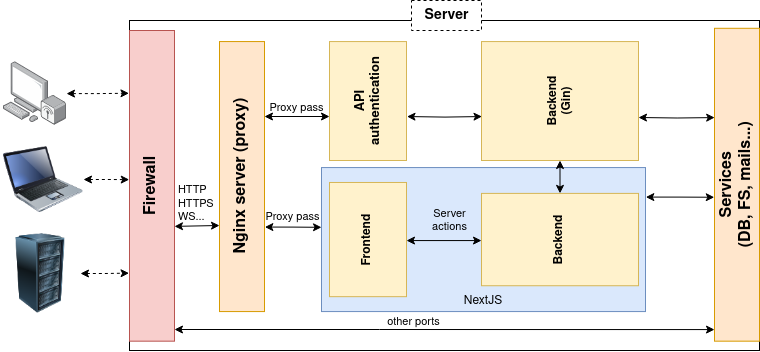
\includegraphics[width=16cm]{files/img/server_scheme.png}
            \caption{Schéma služeb aplikace (AJ)}
            \label{fig:appschema}
        \end{figure}
        
        \section{Backend}
            Na~\acrshort{BE} bude~program v~jazyce \emph{Go}, který zpracovává požadavky od~klienta. Je~dobrou praxí rozdělit kód na~více funkčních celků, tj.~\emph{moduly}. \emph{Moduly} umožňují mmj.~využít veřejně dostupný kód jiných projektů, pokud to dovoluje zadání od~zákazníka i~licence daného \emph{modulu}. Tím~je~možné ušetřit čas, který správa takového modulu zahrnuje~\cite{Zimmerman2023:howtowritebetter}. \emph{Moduly} v~\emph{Go} je~možné používat přímo použitím veřejného odkazu na~zdrojový kód (např.~kód z~\emph{Gitlabu}), čímž~výrazně zjednodušuje práci s~nimi.
            
            Pro~obsluhu požadavků využiji \href{https://github.com/gin-gonic/gin}{\emph{gin-gonic/gin}} s~vlastním dříve~vytvořeným rozšířením o~autentizaci požadavku a~kontrolu a~správu \acrshort{JWT} \href{https://gitlab.com/sjiamnocna/goethe}{\emph{sjiamnocna/goethe}}.

            Při~vývoji využiju nástroj \href{https://github.com/cosmtrek/air}{\texttt{cosmtrek/Air}}, který automaticky restartuje aplikaci při~každé změně kódu, čímž vývoj aplikace zrychlí, jelikož nebude~nutné manuální spouštění aplikace.

            \acrshort{BE} tvoří dvě části, aby~byl~lépe testovatelný a~rozšiřitelný. Jsou to~\emph{webový server}, který bude přijímat požadavky a~zpracovávat uživatelská data, a~\emph{generátor}, který přijme požadavky a~vygeneruje části příkladu podle zadání. Ty~předá ve~strukturované podobě výslednému zobrazení (ve~smyslu \emph{MVC}). V~případě nalezených chyb (např. nekompatibilní nastavení, závislost na~neexistující proměnné\dots), vedoucí k~nevytvoření příkladu, sdělí chyby uživateli, případně se~pokusí, pokud je~to~možné, samostatně chyby odstranit.

            Základním prvkem aplikací je~registrace a~přihlašování uživatelů. Při~registraci je~potřeba ověřit uživatele pomocí e-mailové adresy. Také je potřeba zamezit duplicitním účtům kontrolou existence uživatele před registrací a~uživateli sdělit, že~se pokouší registrovat podruhé, ještě před~odesláním formuláře. Uživatel~se přihlašuje pomocí jména a~hesla nebo~některého \emph{externího poskytovatele ověření identity}.
            
            V~případě, že~uživatel zapomene heslo, je~potřeba mu~poslat e-mail s~odkazem na~stránku, kde~si~může heslo změnit. Tento odkaz musí být unikátní a~platný pouze po~omezenou dobu, aby~nebylo možné jej~zneužít. K~tomu využije jednoznačný \emph{hash}, platný po~omezenou dobu a~obsahující informace o~daném požadavku. Zároveň informaci o~požadavku uložím do~\emph{databáze}, abych mohl po~přístupu na~stránku pomocí odkazu zkontrolovat platnost požadavku na~změnu hesla.

            Šablony s~různými překlady zpráv budou v~adresáři \texttt{/goapp/templates}. Podle jazykových preferencí uživatele se~vybere příslušná šablona. V~případě, že~uživatel nemá nastavený jazyk, použije se~výchozí jazyk, tedy angličtina.
            
        \subsection{Funkce Init}
            \emph{Go} má~dvě vstupní funkce \emph{main} a~\emph{init}. Funkce \emph{main} je~hlavní vstupní bod aplikace, který se~spustí jako první. Funkce \emph{init} se~spustí jako první, ještě~před funkcí \emph{main} a~slouží ke~konfiguraci programu nebo připojení do~databáze. Funkce \emph{main} je~hlavní funkcí aplikace, kde~se nachází logika aplikace volající další akce.

            Ve~chvíli, kdy spustíme aplikaci, se~nejdříve spustí funkce \emph{init} a~poté hlavní část aplikace, funkce \emph{main}.
            
            Funkce \emph{init} použiju k~nastavení připojení k~databázi prostřednictvím \emph{ORM systému} (\href{https://gorm.io/}{\texttt{go-gorm/gorm}}). V~rámci \emph{initu} spouštím migraci databáze, aby \emph{GORM} vytvořil databázové tabulky nebo jejich~podobu aktualizoval. Jednotlivé modely dat jsou vidět ve~zdrojovém kódu aplikace.

            K~připojení do~databáze je~používán tzv.~\acrdefprint{DSN}{Data Source Name}. Je~to~řetezec znaků který obsahuje informace o~připojení do~databáze. Obsahuje \emph{adresu} databáze, \emph{port}, na~kterém běží, \emph{název databáze}, \emph{jméno uživatele} a~\emph{heslo}. Ty~si~načítám z~prostředí systému, tedy \emph{Dockeru}, který si~je~načte ze souboru \texttt{.env}.

            Ve~funkci \emph{init} také přípravuju šablony. Při~použití modulu \texttt{html/template} pro~zpracování šablon s~proměnnými, je~lepší si~šablony připravit do~paměti a~v~místě použití jen~dodat příslušná data. To~zajistí rychlejší odezvu aplikace. Šablony slouží zejména pro~vytváření e-mailů, které budou odesílány uživatelům a~k~tvorbě případných chybových hlášek.

        \subsection{Router}
            Ve~funkci \emph{main} je~hlavní logika aplikace. Spouštím zde~\emph{HTTP server}, který čeká na~požadavky od~\emph{klienta}. K~tomu slouží funkce~\texttt{Run} z~modulu \texttt{gin-gonic/gin}, prostřednictvím mého~dříve vytvořeného modulu \href{https://gitlab.com/sjiamnocna/goethe}{\texttt{sjiamnocna/goethe}}, který zjednodušuje~udržování \emph{JWT tokenu}~--~ověří, načte a~aplikaci zpřístupní informace, které jsou v~tokenu uloženy. Při~každé změně dat změní a~v~odpovědi zašle nový~\emph{token}.
            
            Při~každém volání zkontroluju a~do~požadavku načtu informace o~aktuálním uživateli. S~těmito daty pak~mohou pracovat další \emph{handlery}. Spuštění \emph{Gin} serveru (routeru), nastavení \emph{callbacků} a~vytvoření skupin \emph{endpointů} je~vidět v~kódu~\ref{go:enginerun}.

            Důležitou součástí aplikace \emph{GINu} je~tzv.~\textbf{Router}, který z~příchozího požadavku zjistí, jaký \emph{koncový bod} je~volán a~předá volání~příslušnému \emph{handleru}. \emph{Router} také umožňuje vytvářet skupiny \emph{koncových bodů}, které mají společný základ~\emph{URL} adresy a~které mohou sdílet část logiky. To~umožňuje vytvářet aplikace, které mají jednotnou strukturu a~jsou přehledné. \emph{Router} funguje podobně i~pro obsluhování požadavků na~\acrshort{FE}.


            Obsluha jednotlivých požadavků probíhá v~\textbf{Gorutinách} (\textbf{Goroutines}), což~znamená, že~každý požadavek může být~obsluhován paralelně (zároveň), což~umožňuje obsloužit více požadavků najednou~\cite{effective_go}.

            \begin{code}
                \begin{minted}{go}
                    func main() {
                    	// create gin engine
                    	goethe.Callbacks = &goethe.GCallbacks{
                    		// issueJWT with custom claims
                    		BeforeIssueJWT: callbacks.BeforeIssueJWT,
                    		// verify Service Name and Key
                    		OnVerifyCredentials: callbacks.OnVerifyAPICredentials,
                    		// verify custom JWT claims (e.g. API session)
                    		OnVerifyClaims: callbacks.OnVerifyCustomClaims,
                    	}
                    
                    	engine := goethe.GoetheEntry()
                    
                    	// attach gin-sentry middleware
                    	engine.Use(sentrygin.New(sentrygin.Options{}))
                    
                    	{
                    		// define endpoint groups
                    		categoriesGroup := engine.Group("/Cat", goethe.RequireAuthLevel(goethe.AUTH_USER_LOGGED_IN))
                    		eapp.RegisterCatsGroup(categoriesGroup)
                      
                            //...
                    	}
                    
                    	engine.Run() // listen and serve on 8080
                    }
                \end{minted}
                \caption{Spuštění serveru a definice skupin endpointů}
                \label{go:enginerun}
            \end{code}

            \emph{Endpointy} jsou umístěny v~adresáři \texttt{Endpoints}, kde~má~každá skupina \emph{Endpointů} svůj vlastní adresář. V~těchto souborech jsou jejich \emph{handlery}. \emph{Handler} dostává při~obsluze \emph{požadavku} jako parametr \emph{gin.Context}, který obsahuje kontext aktuálního požadavku a~umožňuje s~ním \emph{handleru} pracovat. Komunikace \acrshort{FE} a~\acrshort{BE} bude probíhat pomocí \emph{JSON}u, případně \emph{HTTP stavovými kódy}. \emph{Endpointy} budou sdružovány podle zdroje se~kterým manipulují, např.;
            \begin{description}
                \item[/api/user]~--~\emph{CRUD} akce přihlášení, registrace a~správy uživatelských účtů, bez~kterých se~neobejde většina moderních aplikací.
                \item[/api/cat]~--~\emph{CRUD} akce spojené s~kategoriemi. Kategorie jsou~určeny pro~zařazení úkolů a~testů nebo~specifikaci konkrétního oboru uživatelem.
            \end{description}

            Při~implementaci načtení dat z~požadavků bylo nutné použít jiný způsob zpracování některých vlastních struktur, jelikož pracuji se~\emph{staticky typovaným} jazykem a~\emph{Gin} nedokázal automaticky zpracovat všechny struktury. Proto načítám danou vlastnost jako textový řetězec a~dále zpracovávám.
            
            Ukázka funkce pro~zpracování struktury dat odpovědí z~\emph{JSON} řetězce na~otázku je~vidět v~kódu~\ref{go:unmarshallanswers};

            \begin{code}
                \begin{minted}{go}
                    // unmarshall data from JSON request byte string
                    func UnmarshallAnswerSlice(raw []byte) ([]generator.Answer, error) {
                    	// single string representation of answer
                    	var answers []struct {
                    		Content  string `json:"Content" binding:"required"`
                    		Correct  bool   `json:"Correct,omitempty"`
                    		MathMode bool   `json:"MathMode,omitempty"`
                    		Generate uint8  `json:"Generate,omitempty"`
                    		Final    bool   `json:"Final,omitempty"`
                    	}
                    
                    	err := json.Unmarshal(raw, &answers)
                    
                    	if err != nil {
                    		return nil, errors.New("wrong format of answers")
                    	}
                    
                    	var res []generator.Answer
                    
                    	// map answers from JSON
                    	for _, ans := range answers {
                    		res = append(res, generator.Answer{
                    			ResultAnswer: generator.ResultAnswer{
                    				Content: ans.Content,
                    				Correct: ans.Correct,
                    			},
                    			Final:    ans.Final,
                    			Generate: ans.Generate,
                    		})
                    	}
                    
                    	return res, nil
                    }
                \end{minted}
                \caption{Načtení dat odpovědí a jejich převod před uložením do databáze}
                \label{go:unmarshallanswers}
            \end{code}

        \subsection{Generátor}
            Zásadní funkci při~tvorbě výsledné podoby zadání bude~mít \emph{generátor}.
            
            Generátor bude postupně nahrazovat hodnoty použitých proměnných a~funkcí ke~generování čísel a~dalších prvků. K~tomuto účelu slouží modul správce proměnných, který nahrazuje proměnné a~funkce jejich hodnotami. Mimo to~zajistí náhodné seřazení a~splnění dalších bodů, které si~uživatel vyžádá. Konečné nahrazení hodnotami proměnných v~zadání proběhne pomocí modulu \texttt{text/template}, který umožňuje jednoduché využití šablon s~proměnnými.
            
            Proměnné budou při~definici i~v~zadání používat stejný zápis jak definuje balík \texttt{template/html}, tedy \texttt{\{\{.jméno\}\}}.

            K~identifikaci proměnných budou sloužit jejich jména. Jména pak~poslouží jako klíče, které na~sebe \textbf{namapují} (přiřadí) vlastnosti a~obsah proměnných. K~určení obsahu, spuštění funkcí, které vygenerují jejich hodnoty, a případnému vyčíslení (redukci) \emph{mnohočlenů} bude nutné vytvořit \textbf{parser}, což~je~program, který bude schopný rozdělit řetězec a~načíst jednotlivé částí, kterým přiřadí konkrétní význam. Podle celkové podoby pak určí, zda jde o~\emph{proměnnou}, \emph{funkci}, \emph{polynom} nebo \emph{operátor/závorku}. U~každé části pak~určí, zda je~platná a~případně ji~nahradí její nalezenou/vypočítanou hodnotou.
            
            \emph{Parser} musí rozložit zápisy hodnot proměnných na~jednotlivé \textbf{dílčí řetězce} (\textbf{tokeny}) a~identifikovat jejich typ. K~tomu použiju modul \href{github.com/bzick/tokenizer}{\texttt{bzick/tokenizer}}. Ten~ve~vstupním textu identifikuje základní typy jako~--~čísla, identifikátory a~vyfiltruje \textbf{bílé znaky} (mezery, ukončení řádku~ap.). Nakonec~vrátí seznam \emph{tokenů}, které v~textu našel. Podle kontextu (typů okolních \emph{tokenů}) potom určím jejich~význam v~aplikaci a~jak je~s~nimi potřeba pracovat.
            
            Např.~pokud za~znakem \{ bude tečka, vím, že~jde o~proměnnou. Pokud je~tam~identifikátor (řetězec znaků) a~závorky s~argumenty pro~funkci, jde o~funkci. Po~zpracování proměnných a~funkcí bude~možné určit zbytek jako~mnohočleny, zlomky~apod.
            
            Při~řešení proměnných musí nejdříve proběhnout spuštění funkcí ve~všech proměnných, na~kterých je~právě řešená proměnná závislá (všechny na~které se~odkazuje). Tím~jsou vygenerovány náhodné nebo~vypočítané hodnoty a~pokud je~proměnná použita na~více místech, bude mít všude stejnou hodnotu. Pro~snížení počtu operací toto provedu při~prvním použití proměnné v~jiné proměnné nebo~v~zadání příkladu.

            Potom je~možné provést nahrazení proměnných, vložením \emph{tokenů} z~proměnné na~místo určení. Pokud je~závislá proměnná definována dříve než~ta~kterou potřebujeme nahradit, jde o~chybu. Pokud závislá proměnná není zpracovaná, zpracuji ji~voláním téže funkce nad~danou funkcí (tzv.~\textbf{rekurzivní volání}). Do~seznamu vložím název proměnné a~pokud zpracovávaná proměnná již~v~seznamu je, jde o~chybu, která by způsobila nekonečné cyklické zpracování týchž proměnných (\textbf{deadlock}).
            
            Proměnné tak~budou nahrazeny ve~správném pořadí a~pokud k~nahrazení nedode, znamená to, že~neexistuje, nebo~má~\emph{cyklickou závislost}.

            V~matematickém režimu je~potřeba~vyčíslit hodnotu výrazu zapsanou v~\emph{tokenech}, např.~\texttt{randInt(0,42) + 1} pro~náhodné liché číslo. To~realizuju pomocí algoritmu podobnému tzv.~\textbf{Postfixové notaci} (\textbf{Reverzní polská notace}), která nevyužívá závorky ani~prioritu operátorů a~operátory jsou zapsány za~operandy. Výraz je~zapsán jako~posloupnost \textbf{operandů} (\textbf{hodnot}) a~\emph{operátorů}, např.~klasický infixový zápis $19 + ( 26 + 1 )$ je~převeden do~\emph{postfixového} jako $19\:26\:1\:+\:+$. Dvojice \emph{operandů} jsou zpracovávány operátorem a~tedy je~jednodušší~zpracování pomocí funkcí (např.\,\texttt{sum(a, b)}) v~programovacích jazycích. Pro~názornost algoritmu převodu a~vyčíslení pomocí struktury \emph{zásobníku} (struktura typu \acrdefprint{LIFO}{Last In First Out}~\cite{Scott2019:programmingpragmatics}) je~možné využít vizualizaci~\href{https://www.free-online-calculator-use.com/postfix-evaluator.html#}{www.free-online-calculator-use.com/postfix-evaluator.html}~\cite{postfixnotation}.

            Protože pracuji s~jazykem \emph{Go}, obdrží \emph{generátor} data ve~formě \emph{struktury} definující příklad a~výsledkem bude~struktura obsahující zpracované zadání a~možnosti s~nahrazenými a~vyčíslenými hodnotami, aby bylo možné hodnoty předat \emph{zobrazení} (ve~smyslu \acrshort{MVC}). Výsledná data budou obsahovat zadání otázky, možnosti odpovědí a~informaci o~tom, která možnost je~správné řešení. Na~místě zobrazení uživatelského vstupu bude vložen \emph{placeholder}, který bude~zpracován až~podle~volby~zobrazení jako vstupní pole nebo~prostor pro~odpověď s~případným výčtem možností.
            
            \emph{Generátor} samotný nemá přístup k~databázi, proto manipulaci se~zadáním a~uložení vygenerovaných hodnot zajistí aplikace v~rámci konkrétního \emph{endpointu}, hodnoty si~načte ze~struktury, kterou obdrží z~generátoru. Konkrétní hodnoty uloží do~databáze vygenerovaných příkladů s~jednoznačným identifikátorem, který předá uživateli, který zároveň bude mít k~dispozici seznam dříve vygenerovaných verzí příkladu a~odkazy na~k~jejich~editaci.

        \subsection{Autentizace uživatelů}
            Registrace a~přihlášení do~aplikace bude možná více způsoby. Pro~všechny způsoby přihlášení bude v~databázi existovat~jedna tabulka s~přihlašovacími údaji. Uživatelé budou moci k~používání aplikace použít kombinaci \emph{e-mailové adresy a~hesla}, ale také \emph{Google} účet, díky použití \emph{Firebase}. V~budoucnu tak~bude~jednodušší přidat i~další služby k~ověření identity uživatele.
            
            Na~\acrshort{FE} použiju nástroj \emph{Firebase} od~společnosti \emph{Google}, který umožňuje mmj.~jednoduchou \emph{autentizaci} uživatelů pomocí účtu u~společnosti Google. Přihlášení pomocí \emph{Firebase} proběhne takto:
            \begin{enumerate}
                \item Uživatel se~přihlásí k~\acrshort{FE} pomocí \textbf{Firebase Authentication}.
                \item \acrshort{FE} vygeneruje \acrshort{JWT} pomocí uživatelských údajů získaných z~\emph{Firebase} a~odešle jej~na~\acrshort{BE}.
                \item \acrshort{BE} (\emph{Go}) ověří \acrshort{JWT} pomocí údaju z~\emph{Firebase}.
                \item \acrshort{BE} najde uživatele v~databázi podle \emph{e-mailové adresy} a~pokud neexistuje, vytvoří nového uživatele.
                \item \acrshort{BE} provede ověření požadavkem na~\emph{Firebase} jménem uživatele a~ověří přihlášení.
                \item \acrshort{BE} vytvoří nový \acrshort{JWT} token a~zašle jej na~\acrshort{FE}.
                \item \acrshort{FE} si~uloží nový \acrshort{JWT} a~uživatele přesměruje do~aplikace.
            \end{enumerate}
            
            Pokud~bude~ověření úspěšné, uživatel je~přihlášen a~unikátní identifikátor aktuální relace vložím do~\acrshort{JWT} a~databáze. Při~každém přístupu bude~zkontrolována platnost relace. To~umožní mít~přehled o~přihlášených uživatelích a~zabezpečí přístup k~datům. Umožní to~načíst data uživatele do~paměti programu a~vzdálené odhlášení v~případě podezřelého přístupu k~účtu.

        \section{Frontend}
            \acrshort{FE} bude vytvořen pomocí nástroje \emph{NextJS} v~jazyce \acrshort{TS}. \emph{NextJS} je~založen na~knihovně \emph{React} a~umožňuje využívat většinu jeho~výhod. Pro~lepší přístupnost a~aplikace znevýhodněmým a~pro~lepší \emph{SEO} využiju k~tvorbě komponent některý z~\emph{CSS} nástrojů nebo hotových šablon, které jsou již~většinou připraveny s~nějakou optimalizací přístupnosti, což~zjednoduší práci při~tvorbě uživatelského rozhrání.

            Pro~komunikaci s~backendem budu používat dříve napsaný \emph{Typescript modul} \href{https://gitlab.com/sjiamnocna/renette-api}{\emph{sjiamnocna/renette-api}}, který je~napsaný k~udržování \acrshort{JWT} a~tedy~zjednoduší komunikaci \acrshort{FE} s~\acrshort{BE}. Při~každé důležité změně, jako přihlášení nebo~odhlášení uživatele se~změní data a~s~nimi i~\emph{JWT token}, čímž se~redukuje riziko jeho zneužití.

            Důležitým bodem při~vývoji je~neukládat citlivé údaje, jako např.~klíče nebo~soukromé údaje v~kódu (tzv.~\textbf{hardcoded}), kde k~nim bude mít~přístup téměř kdokoliv, kdo~má přístup k~používanému verzovacímu systému, a~vzniká tak~riziko zneužití údajů. Proto jsou takové údaje načítány do~systému jako~\textbf{proměnné prostředí} (\textbf{environment variable}). \emph{Docker} je schopný načíst a~zpřístupnit~kontejneru hodnoty, které jsou~uloženy v~souboru \texttt{.env}. \acrshort{BE} napsaný v~\emph{Go} umí~konstanty z~prostředí číst pomocí \texttt{os.Getenv("nazevpromenne")}. Nicméně \emph{NextJS} díky svému návrhu neumožňuje načtení \emph{env proměnných} do~veřejné části aplikace, budu je~při spuštění \emph{NextJS} aplikace pomocí skriptu z~prostředí přepisovat do~\emph{Javascriptového} souboru jako konstanty a~dále s~nimi jako s~běžnými z~\emph{Javascriptu} exportovanými \emph{konstantami} budu~pracovat. Přepis proměnných do~\emph{Javascriptového} souboru bude~prováděn pomocí \emph{Node.js} skriptu, viz~\ref{js:env}.
            
            \begin{code}
                \begin{minted}{js}
                    // node.js environment
                    const fs = require('fs');
                    const os = require('os');
                    
                    // truncate the file and write new env vars into it
                    const f = fs.open('env_vars.js', 'w', function(err, fd) {
                        if (err) {
                            throw 'could not open file: ' + err;
                        }
                    
                        // now one by one write the env vars into the file
                        for (const i in process.env){
                            if (!i.startsWith("NEXT_PUBLIC")){
                                continue;
                            }
                    
                            const content = `export const ${i} = '${process.env[i]}'${os.EOL}`
                            fs.appendFile(fd, content, function(err) {
                                if (err) throw 'error appending file: ' + err;
                            });        
                        }
                    
                        // close the file
                        fs.close(fd, function() {
                            console.log('wrote the file successfully');
                        });
                    });
                \end{minted}
                \caption{Přepis \textbf{env proměnných} na~konstanty pomocí \emph{Node.js} kódu.}
                \label{js:env}
            \end{code}

            Aplikace bude napsaná v~anglickém jazyce, do~ostatních jazyků (vč.~Češtiny) budu aplikaci překládat. K~tomu použiju modul \texttt{next-intl}, který slibuje nativní podporu přímo od~\textbf{Vercelu}. Překlady budou uloženy v~adresáři \texttt{locales} a~budou se~načítat dynamicky podle aktuálního jazyka. V~případě, že~překlad chybí, zobrazí se~anglický text. Překlady budou vytvořeny pomocí \emph{Google Translate} a~budou přeloženy ručně.

            \textbf{Router} v~případě \acrshort{FE} určuje, která stránka (resp.~\emph{komponenta}) bude na~základě \emph{URI} (adresy), \emph{query} parametrů a~stavu okna prohlížeče zobrazena. Veřejná prezentace aplikace bude definována v~hlavní části \emph{routeru}, stránky pro~přihlášené uživatele použijí tzv.~\emph{lazy loading}.

            \emph{React} po~spuštění aplikace normálně načte celou zobrazenou aplikaci naráz, včetně obrázků, obsahu~ap. To~může vyústit ve~zbytečné načítání velkého objemu dat a~ke~snížení celkové rychlosti aplikace, nehledě na~zátěž na~připojení.

            \textbf{Lazy loading} je~technika, umožňující načíst pouze \emph{komponenty}, které jsou potřeba, a~zbytek načítat dodatečně pouze v~případě potřeby. Typicky rozdělujeme funkční komponenty tak, jak~jsou~v~aplikaci použity a~podle toho jsou~postupně načítány. V~této aplikaci budu~používat \emph{lazy loading} pro~načítání stránek, které jsou dostupné pouze přihlášeným uživatelům. V~případě, že~uživatel není přihlášen, bude mu~zobrazena stránka s~přihlašovacím formulářem. V~případě přihlášení uživatele pak~indikuji načítání aplikace a~při~úspěšném načtení zobrazím kontrolní prvky~\cite{lazyload}.

            \emph{Router} je~zodpovědný také za~zobrazení chybové hlášky v~případě, že~uživatel zadá neexistující adresu (\emph{HTTP chyba 404}) nebo~se~snaží k~přístupu ke~stránce, ke~které nemá oprávnění (\emph{HTTP chyba 403}). V~takovém případě je~nutné uživatele informovat, že~došlo k~chybě a~případně mu~doporučit, co~může dělat dál. A~zaznamenat chybu do~logů~--~tj.~\emph{zalogovat}.
            
            \textbf{UI (User Interface)} (\textbf{uživatelské rozhrání}) bude~vytvořeno s~použitím \textbf{Tailwind CSS}. \emph{Tailwind} je~\textbf{utility-first} knihovna -- soustředí~se na~poskytnutí jednoduchých prvků, které je~možné ke~komponentám přidávat jako třídy. Skládáním těchto tříd je~možné vytvořit vzhled, který je~potřeba. \emph{Tailwind} je~také možné rozšířit o~vlastní třídy nebo~další knihovny, které rozšiřují jeho funkčnost a~mohou být~použity v~rámci celé aplikace~\cite{Rappin2022ModernCSSTailwind}.

            K~tvorbě \emph{UI} je~samozřejmě možné použít i~knihovny jako \textbf{Bootstrap}, \textbf{Foundation} nebo~jiné přístupy ke~stylování.

        \section{Testování}
            Nemá význam testovat celý \acrshort{BE}. Balíčky \emph{GIN} i~\emph{GORM} jsou~aktivně testovány při~jejich vývoji. Při~chybě překladu aplikace vůbec nenastartuje, protože selže tvorba \emph{Docker} kontejneru, a~zůstává v~původní funkční verzi. Chyby externích služeb (\emph{SMTP}) jsou~zachyceny v~\emph{Sentry}. Postupem času budu testovací scénáře přidávat a~z~počátku se~budu věnovat testování pouze u~\emph{generátoru} a~\acrshort{FE}, případně \emph{čistých funkcí}.

            Testovány budou všechny scénáře, které jsou od~\emph{generátoru} požadovány~--~např. nahrazení proměnných a~spuštění funkcí, vyčíslení jednoduchých výrazů. Náhodné řazení nelze testovat, protože výsledek je~náhodný a~nelze vyloučit, že~nebudou vygenerovány několikrát stejné hodnoty. Totéž platí pro~náhodné pořadí odpovědí.

            Na~\acrshort{FE} budu testovat funkčnost \emph{komponent}. V~případě, že~se~chyba vyskytne za~běhu aplikace, zaznamená ji~\emph{Sentry} a~upozorní na~nutnost opravy. Díky \emph{Sentry} budu mít informace o~chybě z~\acrshort{FE} i~\acrshort{BE} na~jednom místě a~budu na~ni~včas upozorněn.

        \section{Zálohy}
            \textbf{Zálohování} je~jednodušší díky požití kontejnerů s~\textbf{trvalým úložištěm} (\textbf{volume}), kde~jsou uložena veškerá data, která se~zachovávají i~po~zastavení kontejneru.
            
            Není tedy potřeba zavádět složitý skript pro~zálohování databáze a~všech komponent, pouze pravidelně kopírovat, komprimovat a~na~záložním serveru uschovat data \emph{trvalých úložišť}. Zbytek dat tvoří zdrojový kód, který má~již~zálohu v~podobě \emph{GIT repozitáře}.
        
            
    \chapter{Závěr}
        Cíl práce byl dosažen, podařilo se~vytvořit aplikaci pro~generování školních testů. Koncept aplikace jsem diskutoval s~vybranými učiteli i~vývojáři. Je~také potřeba dodat, že~aplikace je~v~rané fázi vývoje a~některé funkcionality bude nutné ještě dokončit, nicméně aplikace je~již k~dispozici k~použití.
        
        Uživatelé mohou sdílet příklady mezi sebou a~přenechat vymýšlení úloh počítači. Může~tak vzniknout databáze příkladů, která bude moci být~používána k~tvorbě testů. Pokud se~aplikace dostatečně rozšíří, vytvoří databázi generovaných příkladů, kterou budou moci učitelé používat pro~ověření znalostí svých~žáků a~studentů.
        
        V~práci jsem použil aktuální technologie a~postupy a~snažil se~držet základních pouček pro~vývoj aplikací a~psát čitelný, dokumentovaný a~rozšiřitelný kód s~důrazem na~rychlost a~optimalizaci kódu, aby v~budoucnu dokázala obsloužit co~největší počet požadavků.
        
        Je~potřeba vzít v~potaz, že~popsané postupy v~praxi nemusejí být~ideálním řešením a~může~se lišit v~závislosti na~potřebách konkrétní aplikace. V~této implementaci jsem se~soustředil na~vysoký výkon a~ukázku funkce \emph{MVC} s~programem v~jazyce \emph{Go}, nicméně bylo by možné celou aplikaci napsat jednodušeji např.~v~\emph{NextJS}.
        
        Informační technologie se~také neustále vyvíjí a~je~nutné sledovat a~vyhodnocovat nové trendy a~technologie, jelikož v~době publikace této práce již~mohou být~některé postupy překonané. Většina principů ale~zůstane platná.
        
        Výsledná aplikace je~veřejně dostupná na~adrese \href{https://pisemkomat.cz}{\texttt{pisemkomat.cz}}. Kód některých částí aplikace je~možné najít na~Gitlabu (\url{https://gitlab.com/pisemkomat}).

        Bohužel jsem po~mnoha pokusech s~pluginy a~konfiguracemi pro~\emph{I18n} zjistil, že~je~v~\emph{NextJS} již~od~r.~2021 nahlášena chyba (viz~\url{https://github.com/vercel/next.js/issues/21565}), která znemožňuje použití \emph{I18n} zároveň s~konfigurací \emph{proxy} přesměrování. Z~tohoto důvodu bude řešení problému překladů realizováno mimo~rámec této práce a~aplikace je~dočasně zpřístupněna pouze v~anglickém jazyce.

        Aplikace \emph{Písemkomat} je~dostupná také pomocí~\acrshort{API} a~je možné ji~integrovat do~dalších prostředí formou pluginů. Uživatelé tak budou moci používat generované příklady např.~v~prostředí \textbf{Moodlu} nebo~\acrdefprint{CMS}{Content Management System} jako~např.~\textbf{Wordpress}. Dokumentace k~\acrshort{API} je~k~dispozici~ve~veřejné části webu.
        
        Základ pro~tvorbu aplikace pomocí jazyka \emph{Go} a~knihovny \emph{NextJS} je~k~dispozici na~\emph{Gitlabu} \href{https://gitlab.com/gormrest}{\texttt{gitlab.com/gormrest}}. Dokumentace ke~kódu je~realizována pomocí komentářů v~kódu, dokumentačních řetězcích a~souborech \textbf{README} v~popisu repozitářů.

    \clearpage
    \addcontentsline{toc}{chapter}{Seznam použitých zkratek}
    \printglossary[type=\acronymtype, title={\textbf{Seznam použitých zkratek}}]{}
    \clearpage
    
    \addcontentsline{toc}{chapter}{Použitá literatura}

    \renewcommand\bibname{Použitá literatura}
    \bibliographystyle{czechiso}
    \bibliography{zdroje}
\end{document}
